% class
\documentclass[en, oneside, onehalfspacing]{risethesis}

% packages and configurations
\usepackage{enumitem}
\usepackage{lineno, hyperref}
\usepackage[numbers]{natbib}
\usepackage{babel}
\usepackage{supertabular}
\usepackage{fancybox}
\usepackage{acronym}
\usepackage{array}
\usepackage{booktabs}
\usepackage{graphicx}
\usepackage{rotating}
\usepackage{tabularx}
\usepackage{color, colortbl}
\usepackage{multirow}
\usepackage{hhline}
\usepackage{setspace}
\usepackage{placeins}
\usepackage{longtable}
\usepackage{amsthm,amsmath}
\usepackage{mathtools}
\usepackage{algorithm}% http://ctan.org/pkg/algorithms
\usepackage{algpseudocode}% http://ctan.org/pkg/algorithmicx
\usepackage{algpseudocode}
\usepackage{listings}
\usepackage{epstopdf}
\usepackage{subfigure}	
\usepackage{courier}
\usepackage{amsfonts}
\usepackage{morefloats}
\usepackage{lipsum}
\usepackage{cleveref}
\usepackage{hyperref}

\newtheorem{thm}{Scenario}
\hypersetup{breaklinks=true}
\urlstyle{same}
\Urlmuskip=0mu plus 1mu\relax
\lstset{numbers=left, 
	stepnumber=1, 
	firstnumber=1, 
	numberstyle=\tiny, 
	extendedchars=true, 
	breaklines=true,
	frame=tb,
	basicstyle=\footnotesize, 
	stringstyle=\ttfamily,
	showstringspaces=false
}

\definecolor{lightgray}{gray}{0.8}
\definecolor{Gray}{gray}{0.9}
\renewcommand{\lstlistingname}{Code}
\renewcommand{\lstlistlistingname}{Lista de Listagens}

\DeclarePairedDelimiter\abs{\lvert}{\rvert}%
\DeclarePairedDelimiter\norm{\lVert}{\rVert}%
\DeclareMathOperator*{\argmin}{arg\,min}
\DeclareMathOperator*{\argmax}{arg\,max}
\newcommand*\justify{%
	\fontdimen2\font=0.4em% interword space
	\fontdimen3\font=0.2em% interword stretch
	\fontdimen4\font=0.1em% interword shrink
	\fontdimen7\font=0.1em% extra space
	%\hyphenchar\font=`\-% allowing hyphenation
}
	
\address{BRASÍLIA}

\universitypt{Universidade de Brasília}
\universityen{Universidade de Brasília}

\departmentpt{Departamento de Engenharia Elétrica - ENE/FT}
\departmenten{Departamento de Engenharia Elétrica - ENE/FT}

\programpt{Progama de Pós-Graduação em Engenharia Elétrica - PPGEE}
\programen{Progama de Pós-Graduação em Engenharia Elétrica - PPGEE}

\majorfieldpt{Engenharia Elétrica}
\majorfielden{Electrical Engineering}

\title{Discriminative Sensing Based on Signal Processing for Information Security Analysis}
\date{November/2017}

\author{Thiago Pereira de Brito Vieira}
\adviser{João Paulo Carvalho Lustosa da Costa}
% \coadviser{?}

\begin{document}

\frontmatter
\frontpage
\presentationpage

\begin{dedicatory}Ficha Catalográfica\end{dedicatory}

\begin{dedicatory}Signatures\end{dedicatory}

\begin{dedicatory}Dedicatory.\end{dedicatory}

\agradecimentos
First and foremost, I would like to thank God for giving me the life, strength, knowledge and opportunity to undertake this research study and to ..

(...)

Thank You!!

\begin{epigraph}[]{Confucius}
	Wherever you go, go with all your heart.
\end{epigraph}

\resumo
Último passo, por ser um resumo da introduçao, resultados e conclusão.

\begin{keywords}
Discriminative Sensing, Signal Processing, Eigen Similarity Analysis, Tensor Based Dictionary Learning, Critical Factor Analysis, Network Attack Detection, Fraud Detection
\end{keywords}


\abstract
The cost of all types of cyberattacks is increasing for global organizations. The Whitehouse of the U.S. government estimates that malicious cyber activity cost the U.S. economy between US\$57 billion and US\$109 billion in 2016. Recently, it is possible to observe an increasing in numbers of Denial of Service (DoS), botnets, malicious insider and ransomware attacks.

Accenture consulting argues that 89\% of survey respondents believe breakthrough technologies, like artificial intelligence, machine learning and user behavior analytics, are essential for securing their organizations. To face adversarial models, novel network attacks and counter measures of attackers to avoid detection, it is possible to adopt unsupervised or semi-supervised approaches for network anomaly detection, by means of behavioral analysis, where known anomalies are not necessaries for training models.

Signal processing schemes have been applied to detect malicious traffic in computer networks through unsupervised approaches, showing advances in network traffic analysis, in network attack detection, and in network intrusion detection systems. 

Anomalies can be hard to identify and separate from normal data due to the rare occurrences of anomalies in comparison to normal events. The imbalanced data can compromise the performance of most standard learning algorithms, creating bias or unfair weight to learn from the majority class and reducing detection capacity of anomalies that are characterized by the minority class. Therefore, anomaly detection algorithms have to be highly discriminating, robust to corruption and able to deal with the imbalanced data problem.

Some widely adopted algorithms for anomaly detection assume a Gaussian distributed data for legitimate observations, however this assumption may not be observed in network traffic, which is usually characterized by skewed and heavy-tailed distributions.

As a first important contribution, we propose the Eigensimilarity, which is an approach based on signal processing concepts applied to detection of malicious traffic in computer networks. We evaluate the accuracy and performance of the proposed framework applied to a simulated scenario and to the DARPA 1998 data set. The performed experiments show that synflood, fraggle and port scan attacks can be detected accurately by Eigensimilarity and with great detail, in an automatic and blind fashion, i.e. in an unsupervised approach.

Considering that the skewness improves anomaly detection in imbalanced and skewed data, such as network traffic, we propose the Moment-based Robust Principal Component Analysis (m-RPCA) for network attack detection. The m-RPCA is a framework based on distances between contaminated observations and moments computed from a robust subspace learned by Robust Principal Component Analysis (RPCA), in order to detect anomalies from skewed data and network traffic. We evaluate the accuracy of the m-RPCA for anomaly detection on simulated data sets, with skewed and heavy-tailed distributions, and for the CTU-13 data set. The Experimental evaluation compares our proposal to widely adopted algorithms for anomaly detection and shows that the distance between robust estimates and contaminated observations can improve the anomaly detection on skewed data and the network attack detection.

Moreover, we propose an architecture and approach to evaluate a proof of concept of Eigensimilarity for malicious behavior detection on mobile applications, in order to detect possible threats in offline corporate mobile client. We propose scenarios, features and approaches for threat analysis by means of Eigensimilarity, and evaluate the processing time required for Eigensimilarity execution in mobile devices.

\begin{keywords}
Anomaly Detection, Network Attack Detection, Imbalanced Data, Principal Component Analysis (PCA), Eigenvector Similarity, Robust Principal Component Analysis (RPCA).
\end{keywords}


\tableofcontents

\makeatletter
\renewcommand{\@thesubfigure}{\thesubfigure:\hskip\subfiglabelskip}
\makeatother
\setcounter{lofdepth}{2}

\listoffigures
\listoftables

\chapter*{List of Acronyms}
\addcontentsline{toc}{chapter}{List of Acronyms}
\begin{acronym}[]
    \acro{ADM}{Alternating Direction Method}
    \acro{ALM}{Augmented Lagrange Multiplier Method}
    \acro{APG}{Accelerated Proximal Gradient}
    \acro{BYOD}{Bring-Your-Own-Device}
    \acro{C\&C}{Command and Control}
    \acro{CEP}{Complex Event Processing}
    \acro{CF}{Click Fraud}
    \acro{CSF}{Critical Success Factor}
    \acro{DDoS}{Distributed Denial of service}
    \acro{DHCP}{Dynamic Host Configuration Protocol}
    \acro{DNS}{Domain Name System}
    \acro{DoS}{Denial of Service}
    \acro{EDA}{Exploratory Data Analysis}
    \acro{EDC}{Efficient Detection Criterion}
    \acro{EFT}{Exponential Fitting Test}
    \acro{EVD}{Eigenvalue Decomposition}
    \acro{FAM}{Fast Alternating Minimization}
    \acro{FF}{Fast Flux}
    \acro{GETV}{Greatest Eigenvalue Time Vector}
    \acro{GQM}{Goal-Question-Metric}
    \acro{ICMP}{Internet Control Message Protocol}
    \acro{IF}{Isolation Forest}
    \acro{IRC}{Internet Relay Chat}
    \acro{IRLS}{Iteratively Reweighted Least Squares}
    \acro{ISS}{Information Security System}
    \acro{IT}{Iterative Thresholding}
    \acro{HDLSS}{High-Dimension Low-Sample-Size}
    \acro{KNN}{k-Nearest Neighbors}
    \acro{LAC}{Log Analysis Center}
    \acro{LOF}{Local Outlier Factor}
    \acro{MCD}{Minimum Covariance Determinant}
    \acro{MD}{Mahalanobis Distance}
    \acro{MOS}{Model Order Selection}
    \acro{NIDS}{Network Intrusion Detection System}
    \acro{OCSVM}{One-Class Support Vector Machines}
    \acro{PCA}{Principal Component Analysis} 
    \acro{PCP}{Principal Component Pursuit method}
    \acro{PS}{Port Scan}
    \acro{R2L}{Remote to Local}
    \acro{RDA}{Robust Deep Autoencoders}
    \acro{RFE}{Recursive Feature Elimination}
    \acro{RPCA}{Robust Principal Component Analysis}
    \acro{SVM}{Support Vector Machines} 
    \acro{TCP}{Transmission Control Protocol}
    \acro{TCU}{Federal Court of Accounts}
    \acro{TIM}{Threat Intelligence Manager}
    \acro{U2R}{User to Root}
    \acro{UAL}{User Activity Logging}
    \acro{UDP}{User Datagram Protocol}
\end{acronym}
\mainmatter

% Introdução: cenario, motivacao, problema, solucoes atuais, escopo do trabalho, lista de contribuicoes, organizacao do resto do artigo. 
% Chapter Structure
% 	Motivation
% 	Problems Statement
%	Contributions
% 	Dissertation Organization
\chapter{Introduction}
\label{ch:1_introduction}

\begin{quotation}[]{Lao Tzu}
The softest things in the world overcome the hardest things in the world.
\end{quotation}


\section{Motivation}
\label{sc:motivation}

Traditionally, cyber defense methods can be effective against ordinary and conventional types of attacks, yet may fail against innovative malicious techniques \cite{lakhina2005mining}. In order to be able to detect and avoid novel attacks and their variations, it is necessary to develop or improve techniques to achieve efficiency on resource consumption, processing capacity and response time. Moreover, it is crucial to obtain high detection accuracy and capacity to detect variations of malicious patterns. Recently, signal processing schemes have being applied to detect malicious traffic in computer networks \cite{Lu2009,Huang2009,Zonglin2009,david2011blind,da2012improved,tenorio2013greatest, vieira2017model}, showing advances in network traffic analysis.

Information security may consist of both technical and procedural aspects. The former includes equipment and security systems, while the latter corresponds to security rules and recommendations of good practices. Intrusion detection and intrusion prevention systems are security systems used, respectively, to detect (passively) and prevent (proactively) threats to computer systems and computer networks. Such systems can work in the following fashions: signature-based, anomaly-based or hybrid \cite{Huang2009,mudzingwa2012study}.

Anomaly detection can be defined as the identification of rare and suspicions events by differing the normal or majority of the data. Anomalies are also referred to as outliers, novelties, noise or deviations, and can be related to network attacks, frauds or defects \cite{bhuyan2014network,ahmed2016survey}. Additionally, anomaly detection techniques can be categorized in classification, statistical, information theory and clustering based, according to \cite{bhuyan2014network,ahmed2016survey,osanaiye2016distributed}. Anomalies can be hard to identify and separate from normal data due to the rare occurrences of anomalies in comparison to normal events, therefore anomaly detection algorithms have to be high discriminative, robust to contamination and able to deal with the imbalanced data problem \cite{he2008learning}.

Several efforts and researches aim to avoid network attacks based on known attackers, fingerprints or behavioral analysis. However, distributed attacks organized by botnet has increasing and demanding the development of counter measures in order to detect and avoid unknown attacks or even to deal with adversarial changes on behavior, location and other patterns, in order to avoid detection by behavioral or pattern based detection systems \cite{gu2008botminer, garcia2014empirical,khattak2015botflex,acarali2016survey,wang2017botnet,Wang2018ddosbotnetssurvey}. To face this problem, it is possible to adopt unsupervised or semi-supervised approaches for network anomaly detection, where it is not necessary known anomalies for training models \cite{moustafa2019holistic}.

Recent developments in science and technology have enabled the growth and availability of raw data to occur at an explosive rate. This has created an immense opportunity for knowledge discovery and data engineering research to play an essential role in a wide range of applications from daily civilian life to national security. Despite the actual high availability of information, the relevant information of some observations is generally of under much reduced dimensionality compared to available data sets. The extraction of relevant information by identifying the generating causes within classes of signals is useful for classification problems and for security analysis. 

The high availability of raw data increases the challenges related to big data analytics and to imbalanced learning problems, which corresponds to data sets exhibiting significant imbalances of classes or rare events of some classes. The fundamental issue with the imbalanced learning is the ability of imbalanced data to significantly compromise the performance of most standard learning algorithms. Data analysis of imbalanced data is challenging for classification and prediction problems related to anomaly detection, novelty detection, fraud detection and attack detection.

Some widely adopted algorithms assume a gaussian distributed data, however this assumption may not be observed in real world problems, such as the case of network traffic analysis, where network traffic features are usually more characterized by skewed and heavy-tailed distributions \cite{lakhina2005mining,benson2010network,leon2017probability}. It was observed that the skeweness and heavy-tailed distributions can impact algorithms that rely on gaussian distributed data, as well as it can reveal characteristics that can be exploited in order to obtain accurate classifiers for network anomaly detection.

\section{Problem Statement}
\label{sc:problems}

Considering the above described landscape, this thesis outlines the development and evaluation of approaches based on subspace learning for network attack detection, through methods to make the data discriminative and able to identify structures, hidden patterns and the most relevant information for anomaly detection. In the Subsection \ref{sc:Hypothesis} we present our hypothesis formulation and the Subsection \ref{sc:proposals} describes the proposals to answer the questions and validate the hypotheses.

\subsection{Hypothesis Formulation}
\label{sc:Hypothesis}

For the experimental evaluation of our proposals, we adopt a methodology based on aspects of GQM (Goal-Question-Metric) template \citep{Basili1994} and define two questions to achieve our goal, which are:

\begin{itemize}
	\item $Q_1$: Can the analysis of patterns from a learned subspace identify and detect anomalies in network traffic?
	\item $Q_2$: Can the robust subspace learning improve the anomaly detection in imbalanced and skewed data?
\end{itemize}

Our testing hypotheses are defined in Table \ref{tab:hypothesis}, that describe the null hypothesis and alternative hypothesis for each previously defined question. 

\begin{table}[htb]
	\centering
	\caption{Hypotheses to evaluate the defined metrics}
	\label{tab:hypothesis}
    \begin{tabular}{|p{6cm}|p{6cm}|c|} \hline
        \textbf{Alternative Hypothesis}	&\textbf{Null Hypothesis}	&\textbf{Question} 	\\ \hline
        $H_{1sub}$: It is possible to use subspace learning to identify and detect anomalies in network traffic.
        &$H_{0sub}$. It is not possible to use subspace learning to identify and detect anomalies in network traffic.	&$Q_1$\\ \hline
        $H_{1rob.sub}$: The robust subspace learning improves the anomaly detection from imbalanced and skewed data.	&$H_{0rob.sub}$. The robust subspace learning does not improves the anomaly detection from imbalanced and skewed data.	&$Q_2$\\ \hline
    \end{tabular}
\end{table}

The hypotheses $H_{1num.indct}$ and $H_{0num.indct}$ were defined to evaluate if a subspace learned by singular value decomposition are sensitive to outliers and can be used to detect network attacks. We defined the hypotheses $H_{1scale.prop}$ and $H_{0scale.prop}$ to evaluate the feasibility and performance of a robust subspace learned by Robust PCA to network anomaly detection. 

The metrics most adopted to evaluate experimental results of network attack detection are the true positive (TP), true negative (TN), false positive (FP) and false negative (FN). We adopt these metrics and also adopt the misclassification rate and the F1-score, which is the preferable measure for imbalanced data sets \cite{powers2011evaluation,moustafa2019holistic}.

\subsection{Proposals}
\label{sc:problem_statement}

In the context of anomaly-based schemes, this thesis proposes the Eigensim, which is a approach based on subspace learning techniques for detection of malicious traffic in computer networks. 

Inspired by \cite{david2011blind,da2012improved}, Eigensim models the network traffic using a signal processing formulation as a composition of three components: signal, artifact and noise, taking into account the incoming and outgoing traffic in certain types of network ports (TCP or UDP). The proposed technique is based on eigenvalue analysis, model order selection (MOS) and similarity analysis. In contrast to \cite{david2011blind,da2012improved,tenorio2013greatest}, MOS and eigenvalue analysis are applied to detect detailed time frames under attack. We evaluate the accuracy and performance of the proposed framework applied to a experimental scenario and to the DARPA 1998 data set \citep{osanaiye2016distributed}, which is a well known network traffic data set. Furthermore, this proposed approach is validated into a prove of concept regarding behavioral anomaly detection to detect possible threats to a offline corporate mobile app. 

Network anomaly detection problems are usually characterized by skewed and imbalanced data \cite{Phua2004minority,he2008learning,benson2010network}. Learning algorithms for imbalanced data has been a challenging research topic, considering that the fundamental issue with the imbalanced learning problem is the ability of imbalanced data to significantly compromise the performance of most standard learning algorithms \cite{he2008learning}. 

Some widely adopted algorithms assume a gaussian distributed data, however this assumption may not be observed in real world problems, such as the case of network traffic analysis, where network traffic features are usually more characterized by skewed and heavy-tailed distributions \cite{lakhina2005mining,benson2010network, leon2017probability}. Therefore, the skeweness and heavy-tailed distributions can impact algorithms that rely on gaussian distributed data, as well as it can be exploited to reveal characteristics that can improve classifiers for network anomaly detection. 

We believe that the skewness of anomalous and normal data can highlight features for improving anomaly detection in imbalanced data. We also believe that the distance between robust estimates of normal and contaminated data can highlight discrepancies and be used anomaly detection and for network attack detection. Therefore, we propose the m-RPCA, which is an approach based on  distances of moments computed from a robust subspace learned by RPCA, for anomaly detection on imbalanced and skewed data.

\section{Contributions}
\label{sc:contributions}

We analyze problems related to detection of information security issues and propose new approaches to improve malicious behavior detection through signal processing techniques based on subspace learning. The results of the work presented in this thesis provide the following contributions:

\begin{enumerate}
	\item We propose an approach based on eigen similarity analysis for extracting detailed information about accurate time and network ports under network attack, and evaluate the accuracy and performance of the proposed framework applied to an experimental scenario and to the DARPA 1998 data set;
	\item We discuss the computational complexity of the proposed framework and evaluate the required processing time for tested scenarios;
	\item We propose an architecture and techniques for offline behavioral analysis of a corporate mobile client security architecture, and discuss the processing time of the proposed framework for mobile devices;
	\item We propose an approach based on distances of moments computed from a robust subspace learned by RPCA, for anomaly detection on imbalanced and skewed data, and evaluate the anomaly detection rate on synthetic and real data sets;
\end{enumerate}

\section{Thesis Organization}
\label{sc:organization}

This thesis is organized as follows. In Chapter \ref{ch:2_mos_eig_sim}, we propose the Eigensim, which is an approach based on signal processing techniques for detection of malicious traffic in computer networks, based on eigenvalue analysis, model order selection (MOS) and similarity analysis. Chapter \ref{ch:3_mobile} presents a prove of concept regarding the evaluation of an approach and architecture based on user behavior analysis through the Eigensim  \cite{tenorio2013greatest}, in order to detect threats in a mobile application. Chapter \ref{ch:4_m_rpca} proposes the m-RPCA, which is an approach based on distances of moments computed from a robust subspace learned by RPCA, for anomaly detection on imbalanced and skewed data. Chapter \ref{ch:5_conclusionfuturework} draws the conclusions and the suggestions for future work. Furthermore, the Appendix \ref{apx:a_mos} presents mathematical concepts of examples of state-of-the-art MOS schemes and the Appendix \ref{apx:b_csf_fs} presents a critical factors analysis based on Principal Component Analysis (PCA) for visual discriminant analysis, and presents an approach based on Recursive Feature Elimination (RFE) combined with Support Vector Machine (SVM) \cite{hearst1998support}, applied to the survey that evaluates the IT governance of Brazilian public organizations, in order to identify the Critical Success Factors (CSF) for IT governance of the public sector according to TCU.
\include{chapters/2_eigen_similarity/eigen_similarity}
%%%%%%%%%%%%%%%%%%%%%%%%%%%%%%%%%%%%%%%%%%%%%%%%%%%%%%%%%%%%%%%%%%%%%%%%%%%%%%%%%%%%%%%%%%%%%%%%%%%%%%%%%%%%%%%%%%%%%%%%%%%%%%%%%%%%%%%%%
% Abstract: dar uma idéia dos principais resultados encontrados. 
% Introdução: cenário, motivacao, problema, solucoes atuais, escopo do artigo, lista de contribuicoes, organizacao do resto do artigo. 
% Trabalhos Relacionados: fazer uma das duas coisas a seguir (ou as duas): 
%	a) quando citar uma ou um grupo de referencias relacionado an um tema especifico, conclua o paragrafo mostrando a diferenca para a proposta a ser descrita. 
%	b) no final da secao, compile todas as diferenças e deixe explicito as contribuicoes novamente.
% Metodologia: coloque uma figura para ilustrar todo o processo de coleta e analise. coloque numa tabela (ou mais de uma) a descricao das metricas de interesse, alem dos fatores e niveis selecionados em outra tabela. explique o motivo desses fatores influenciarem as metricas de interesse.
% Conclusão: evite apresentar os resultados mais fáceis de concluir. bons revisores olham o casamento do que vc escreve no abstract/introdução com a conclusao, então mantenha coerente an introdução com a conclusão. Em geral, resultados que sao aparentemente obvios - nao eram até vc mostrar :) - enfraquecem as outras contribuicoes. p.ex, "Os resultados mostraram que o MapReduce apresenta uma boa solução para utilizar computadores comuns para obter alta capacidade de processamento e lidar com an análise massiva de tráfego de rede." pode ser reformulado ou retirado da conclusao. 
\chapter{Eigensim for Anomaly Detection in Offline Mobile Client}
\label{ch:3_mobile}

\begin{quotation}[]{Confucius}
Life is really simple, but we insist on making it complicated.
\end{quotation}


The protection scheme used in a mobile device should be both computationally secure as well as resource-constrained due to battery power limitations \cite{khan2015cloud}. Therefore, encrypting files and generating keys on a mobile device is not considered a good solution. On the other hand, the protection schemes with good computational qualities lack the security analysis in many cases \cite{khan2014bss}. The common practice is the shadow user activities monitoring \cite{yovel2014}. However, the mobile device usage stays unprotected in all the proposed scenarios while in offline mode. When the mobile client goes offline with the sensitive corporate data on board all powerful cloud-based tools can not help and the mobile client has to secure itself with its own limited resources. Moreover, due to the resources constraint, there is a crucial difference in strategy of online and offline mode protection.

Additional security issues and requirements have to be considered when mobile clients are actively used in corporate cloud environment \cite{yovel2014}. Today more and more organizations and enterprises are functioning in the Bring-Your-Own-Device (BYOD) paradigm. The uncontrolled usage of the mobile devices represents a serious risk to the development of secure SME cloud platforms being the bottleneck of the corporate information security system (ISS). While the enterprise cloud infrastructure based on the web interface can be protected by powerful third-party services, such as CASB and CAC, the corporate mobile client is usually light-weighted and generally less protected. 

This work proposes an architecture and approach for user behavior analysis based on Eigensim \cite{vieira2017model}, in order to detect possible threats in offline corporate mobile applications. The key expiration period is safely incorporated into the proposed system solution in order to enhance security and the behavioral analysis can indicate malicious behaviors, their variations, as well as novel attacks, which present low or high variance in comparison to legitimate user behaviors.

The work is structured as follows. Section \ref{sec:3_related_works} analyzes the most common security problems in the mobile cloud environment and the solutions for offline protection in the BYOD world. Section \ref{sec:3_the_client_security_architecture} outlines the mobile security architecture of the proposed solution. Section \ref{sec:3_offline_mode} presents the detailed scheme of the proposed solution to the problem of offline mobile client security. Section \ref{sec:3_eigensim} explains the use of Eigensim. Section \ref{sec:3_results} discusses the common threat scenarios, the data modeling, the performance analysis and discussion of the practical implementation results. Section \ref{sec:3_conclusion} concludes the chapter.


\section{Related works}
\label{sec:3_related_works}

The increasing usage of BYOD demands more sophisticated data protection services compared to ordinary computing environment. A common practice is to provide additional contextual methods apart from authentication, DLP services, and encryption, which can be at rest, in transit and in use \cite{yovel2014, khan2015cloud, khan2014survey, khan2013towards}. The contextual methods increase the security of the mobile client at a maximum level with minimum resource requirements. The most commonly used are:

\begin{enumerate}
	\item Using geolocation of the device to trace its usage;
	\item Setting up the expiration period of an app;
	\item Setting up the expiration period of client pass pin;
	\item Setting up the counter of failed tries;
	\item Secured transfer politics between apps;
	\item Restricting access to the corporate app;
	\item Restricted or prohibited offline access;
	\item Logging and auditing.
\end{enumerate}

Preventing data leakage on the mobile device is a crucial security problem. Therefore, it is necessary to take additional control and protection measures for the confidential data on the mobile devices that leave the boundaries of the organization. Generally, the most sensitive and confidential data should not be permitted to be transferred to the mobile device. However, what if the SME need to allow their employees to work on such devices and even use them on the offline mode for the convenience and traffic reducing, or even for a particular characteristic of the mobile client or the business itself?

From the theoretical point of view of this problem, there are several surveys, whose common point is the mobile cloud as a rapidly developing paradigm that poses many security and complexity problems \cite{khan2013towards, yovel2014, khan2014survey, khan2015cloud, mayrhofer2015architecture, chang2015design, xia2015tinman, kulkarni2015addressing, shila2016amcloud, heydari2016efficient}. Kulkarni and Khanai \cite{kulkarni2015addressing} discuss the most important threats related to Mobile Cloud Computing and argue that there is a need for a lightweight secure framework that provides security with minimum communication and processing overhead on mobile devices. 

An analysis of the new models of mobile cloud computing and new ways of using data storage services is presented in \cite{khan2015cloud, khan2013towards, mayrhofer2015architecture, chang2015design}. Commonly, the models and protection schemes concentrate on the encryption properties and either perform the computations on their own \cite{zhao2010trusted, yang2011provable} or use the cloud provider to off-load the cryptographic operations \cite{itani2010energy, ren2011lightweight}. Obviously, it is natural the mobile client cannot handle all operations securely without the assistance of a cloud provider, due to resources constraint and battery limitation.

The necessity to use schemes that function without putting load on a provider arises when it is desired to make the mobile client less dependent on the cloud provider, i.e. corporate client continues to provide the secure access to the sensitive data without connection to the network. As discussed in \cite{khan2015cloud}, all the currently known schemes of encryption, performing the computation, either use a cloud provider \cite{zhao2010trusted}, a third party trusted agent \cite{yang2011provable, heydari2016efficient}, a combination of both \cite{itani2010energy} or ad hoc approaches \cite{shila2016amcloud}. In some cases, they concentrate on computational complexity without taking care of user privacy and security \cite{ren2011lightweight}. Therefore, according to \cite{khan2013towards, khan2015cloud}, the state-of-the-art mobile cloud security models do not consider the problem of the offline security mode. 

To the best of our knowledge, the offline mode security problem has not yet been deployed, neither in academia nor in the industry \cite{yovel2014, khan2015cloud, khan2014survey, khan2013towards}. Therefore, the main concern of this proposal is the protection of the mobile client and its data in offline mode, when the functions of data protection cannot be offloaded to a cloud or a trusted party. 

\section{The mobile security architecture}
\label{sec:3_the_client_security_architecture}

The approach proposed in this work describes and implements a mobile client security infrastructure for malicious behavior analysis. The mobile security processes depend on the key expiry period, and are used to access the protected storage. Once the user keys expire, the user is requested to enter his valid credentials, i.e. PIN and password. The mobile client then sends the credentials to the server for verification. Once the new set of access keys is received, the user can access the protected files in the offline mode, without the access to the server. This means that no further communication with the server is needed until the key expires. 

The core set of functions and protocols of the proposed architecture can be divided into three sets of operations as shown in Figure \ref{fig:3_01}.

\begin{figure}[h!]
	\centering
	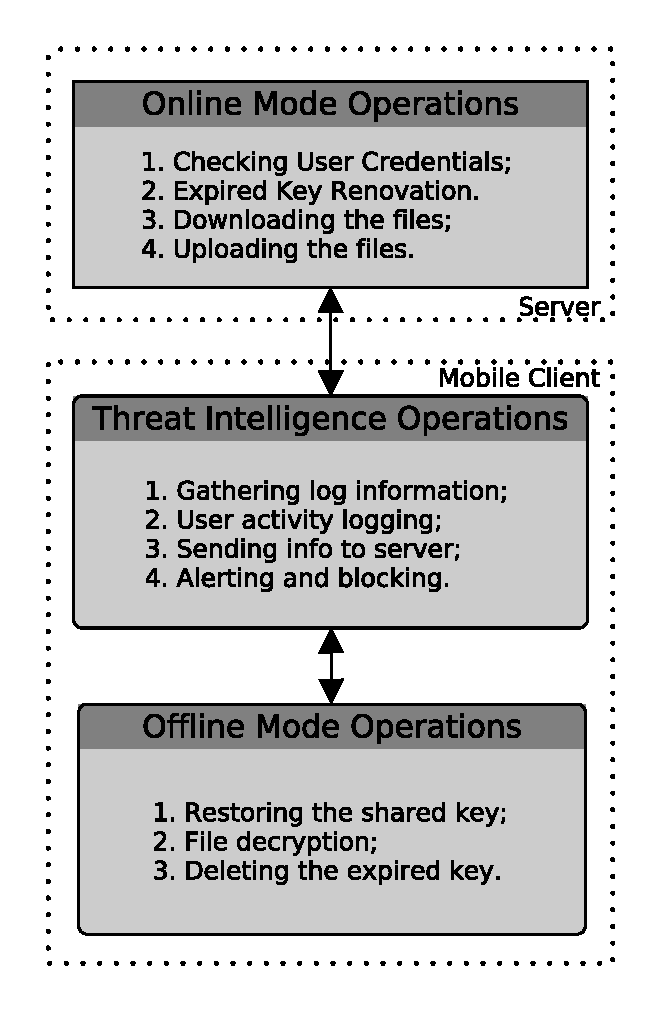
\includegraphics[width=8cm]{figures/ch3/fig01.eps}
	\caption{The core set of functions and protocols of the mobile cloud security infrastructure}
	\label{fig:3_01}
\end{figure}

Figure \ref{fig:3_01} describes the mobile client protection both in online and offline mode. In online mode, the client has the possibility to connect to the server and the security of the client is enhanced by the server-backed up mechanisms. On the other hand, in offline mode the client’s security is supported by the standalone mechanisms. Additionally, the mobile client protection is enhanced by the threat intelligence unit providing the constant monitoring and analysis.

Figure \ref{fig:3_02} depicts the client-side protection mechanisms. The client should support 4 subsystems: 
\begin{enumerate}
	\item Encryption subsystem that provides the procedures of encryption and decryption;
	\item Protected storage subsystem that provides the downloaded shares and key storage protection;
	\item The Threat intelligence unit that provides the constant monitoring;
	\item The communication subsystem that enables with the server.
\end{enumerate}

In summary, all security procedures are connected to 4 groups of operations: file request and receiving; encryption and decryption; file and key storing; monitoring and analysis.

\begin{figure}[h!]
	\centering
	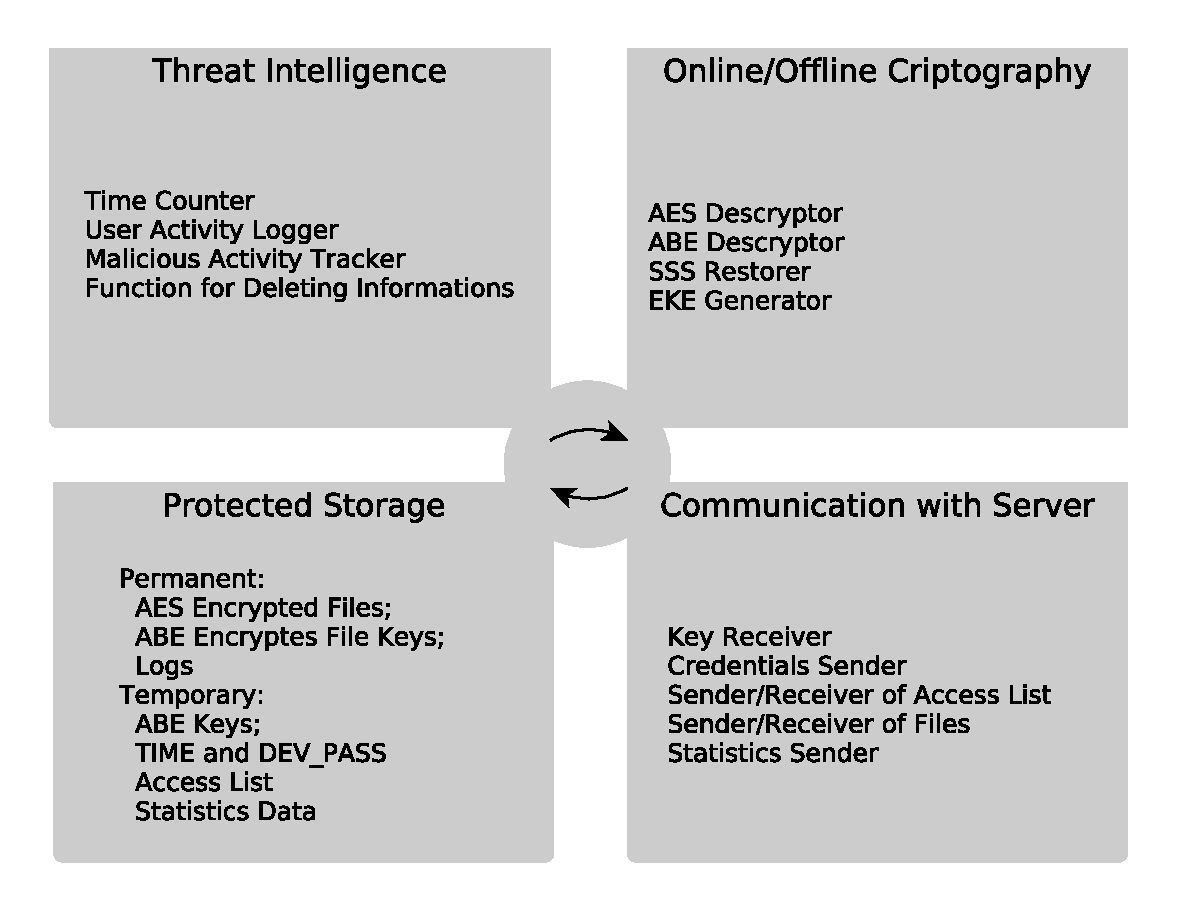
\includegraphics[width=12cm]{figures/ch3/fig02.eps}
	\caption{The Client-side Architecture}
	\label{fig:3_02}
\end{figure}

This architecture consists of the modules of cryptographic functions, threat intelligence infrastructure, communication with server and storage. However, this work focus on the threat intelligence infrastructure module for malicious behavior analysis.

The threat intelligence infrastructure takes into account simple actors such as the time counter for the key expiry period, the counter of unsuccessful tries in order to protect from brute force attacks, and Eigensim-inspired statistics analyzer. Functions such as alerting and deleting the expired key belong to this module as well. These functions are described in Subsection \ref{sec:3_eigensim}.

\section{The proposed solution for offline mobile security}
\label{sec:3_offline_mode}

This section proposes an approach for the mobile client protection in which the security is supported in offline modes. Currently and to the best of our knowledge, the systems of mobile client protection follow a model where the protected client can operate only when it is connected to the cloud, which is not always convenient for the end-user. The basic principles of the mobile client protection herein proposed are: 

\begin{enumerate}
	\item Optimized communication with the cloud when the mobile client does not need to be constantly connected to the server due to the resource constraint and necessity to secure this communication;
	\item Optimized combination of the security mechanisms so that the mobile client does not need to perform complex computation like encryption and key generation due to its resource constraint;
	\item Behavioral analysis of user's operations on mobile client, which can indicate anomalous or automated activities performed by attackers.
\end{enumerate}

The most important security issues in the proposed model arise when the client goes to the offline mode and the user is still allowed to get the access to the protected SME documents. In this case, the server can neither monitor the user activity nor provide the protection methods. The security should be performed at the mobile client. Additionally, the maximum protection should be provided at the minimum resource cost. 

In the online mode the mobile client uses the secure communication with the server in order to verify the validity of user’s credentials. On the contrary, the offline protection model should be approached independently.

\begin{figure}[h!]
	\centering
	\includegraphics[width=15cm]{figures/ch3/fig03.eps}
	\caption{Proposed Architecture for Offline Mobile Security}
	\label{fig:3_03}
\end{figure}

The Figure \ref{fig:3_03} describes the proposed architecture for offline mobile security, showing the modules responsible for securing the mobile client, which includes:

\begin{enumerate}
	\item \pmb{Protected Storage}: the storage is protected with the shared user key and contains the ABE keys giving access to the file keys which allow decrypting the stored files.
	\item \pmb{Threat Intelligence Manager (TIM)}: most attacks incur into significant variation on the legitimate behavior of information systems, or they adopt well-known patterns that can be easily detected by monitoring the system in the case of the offline mode. Signal processing techniques have been successfully applied to anomaly detection \cite{lu2009network, huang2009signal,vieira2017model} and have become a solution to a problem of improving detection accuracy, adaptability and computational cost for application on resource-constrained scenarios. Therefore, signal processing can be applied in offline mobile client security, for evaluating anomalies on user's behavior, according to the scenarios in Section \ref{sec:3_results}. Moreover, the Eigensim, which is an approach based on subspace learning and on effective signal processing technique to separate noise components from the principal components, named Model Order Selection (MOS), can be applied into anomaly and attack detection \cite{tenorio2013greatest, vieira2017model}, to identify and separate malicious behaviors from the legitimate ones. The TIM is an internal module of the mobile client that implements offline anomaly detection through signal processing techniques.
	\item \pmb{Key Management Center}: it includes the functions for maintaining the key expiry period and deleting the expired keys. 
\end{enumerate}


\subsection{Offline Behavioral Analysis}
\label{sec:3_offline_behavioral_analysis}

In the proposed client security architecture, the Threat Intelligence Manager (TIM) is responsible for receiving logged user operations, perform feature extraction, data modeling and malicious behavior analysis in order to identify possible threats, in offline mode. Figure \ref{fig:3_06} depicts the TIM workflow for offline behavioral analysis. 

\begin{figure}[h!]
	\centering
	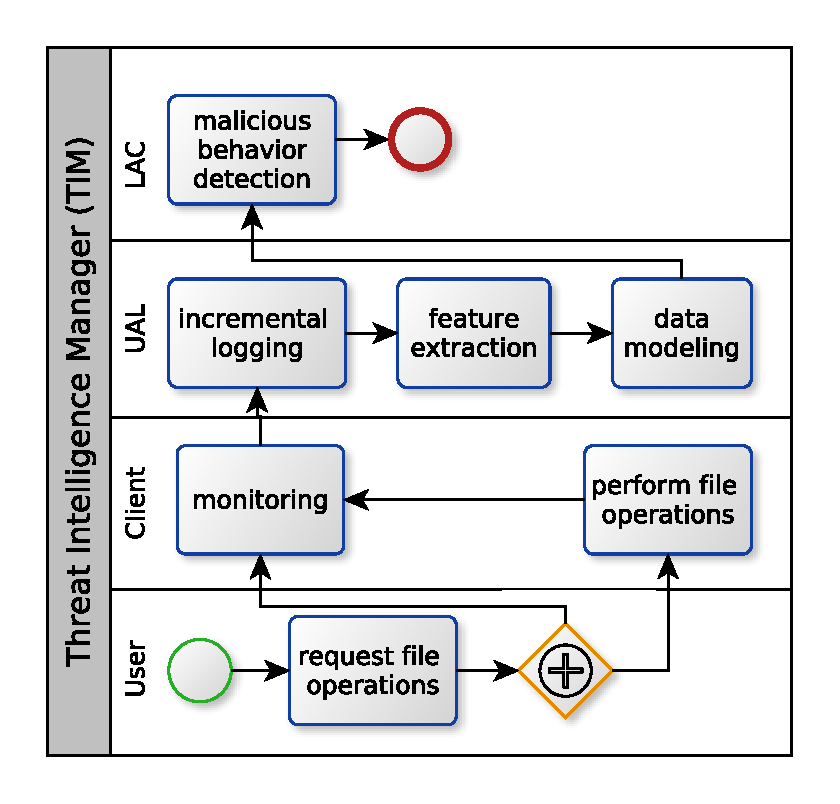
\includegraphics[width=10cm]{figures/ch3/fig06.eps}
	\caption{The Threat Intelligence Manager Workflow}
	\label{fig:3_06}
\end{figure}

As depicted in Figure \ref{fig:3_06}, users request operations are logged so that the main features can be monitored in the mobile client. The user behavior, trying or effectively executing operations, shall be incrementally captured and logged, making possible to monitor the main features that can reveal malicious behaviors, as well as to identify unexpected behaviors that can reveal possible threats. Therefore, the user operations are monitored by the client app, which sends the information to the User Activity Logging (UAL). 

The UAL is responsible for the incremental logging of activities of the mobile client, feature extraction and data modeling for malicious behavior detection, through the Log Analysis Center (LAC). As an internal module of the mobile client, the UAL implements monitors of selected events of the application, such as a login attempt or a file decryption, and logs the desired information for further analysis. The logged information shall be decomposed into selected features and modeled as matrices, composed of the number of occurrences of the selected features by its location and by time. The resultant data is submitted to the LAC, for anomaly detection.

The LAC performs the behavioral analysis through eigenvalue analysis and MOS schemes proposed by Eigensim, which identify anomalies on sparse, subtle or abrupt number of user operations. The malicious behavior detection is detail described in \ref{sec:3_eigensim}.

\section{Eigensim for Threat Intelligence}
\label{sec:3_eigensim}
In the context of anomaly-based schemes for attack detection, the proposed behavioral analysis approach applies signal processing techniques, such as subspace learning by eigenvalue decomposition and Model Order Selection schemes \cite{tenorio2013greatest}, for automatic detection of attacks or malicious behaviors. Model Order Selection is an effective signal processing technique for several applications, allowing separating the only noise components from the principal components applying a rank reduction of the data. 

Applying MOS to the analysis of user operations can be effective in order to reveal the occurrence of malicious behavior during an offline session. MOS for threat intelligence requires that the target features, such as user operations, should be modeled as a matrix composed by the number of occurrences grouped by location and time, and splited into $Q$ time frames. Therefore, the framework considers the time variations of the matrix $\pmb{X}^{(q)} \in \mathbb{R}^{M\times{N}}$, with $q = 1, \ldots, Q$, in order to detect the occurrence of malicious behaviors. For example, one element of $\pmb{X}^{(q)}$ can represent the number of file readings on folder $m$ during the minute $n$, from file operations logged by the mobile client.

The Eigensim can rely on sample covariance of zero mean variables (called as \pmb{zero mean covariance} for the sake of simplicity) and sample covariance of zero mean and unitary standard deviation (called as \pmb{zero mean and standardized covariance} for the sake of simplicity) variables, where the former is useful to identify abnormalities caused by large amounts of operations during a period, while the latter is applied to identify anomalies on sparse or subtle number of file operations.

Classical approaches to model order selection require the computation of the sample covariance matrix $\hat{\pmb{R}}_{yy}^{(q)}$ and of its eigenvalues, obtained from the measurement matrix $\pmb{X}$ of the zero mean samples given by

\begin{equation}\label{eq:3.03}
	\pmb{y}_{m}^{(q)} = \pmb{x}_{m}^{(q)} - \bar{\pmb{x}}_{m}^{(q)}.
\end{equation}

The set of obtained vectors $\pmb{y}_{m}^{(q)}$ composes the zero mean matrix $\pmb{Y}^{(q)}$, then the zero mean covariance matrix $\hat{\pmb{R}}_{yy}^{(q)}$ can be estimated as follows

\begin{equation}\label{eq:3.04}
	\hat{\pmb{R}}_{yy}^{(q)} = \frac{1}{N}\pmb{Y}^{(q)}\pmb{Y}^{(q)^{\rm T}},
\end{equation}
where $\hat{\pmb{R}}_{yy}^{(q)}$ means the estimation of the sample covariance matrix from the measured zero mean matrix $\pmb{Y}^{(q)}$ over $N$ minutes of the time frame $q$. 

For Eigensim based on sample covariance of zero mean and unitary standard deviation, in order to identify anomalies with sparse or subtle behavior, it is required, for each variable, to make the standard deviation unitary as follows

\begin{equation}\label{eq:3.05}
	\pmb{z}_{m}^{(q)} = \frac{\pmb{x}_{m}^{(q)} - \bar{\pmb{x}}_{m}^{(q)}}{\pmb{\sigma}_{m}^{(q)}}.
\end{equation}

The set of vectors $\pmb{z}_{m}^{(q)}$ composes the matrix $\pmb{Z}^{(q)}$, then the zero mean and standardized covariance matrix $\hat{\pmb{R}}_{zz}^{(q)}$ can be calculated via 

\begin{equation}\label{eq:3.06}
	\hat{\pmb{R}}_{zz}^{(q)} = \frac{1}{N}\pmb{Z}^{(q)}\pmb{Z}^{(q)^{\rm T}}.
\end{equation}

Once the $\hat{\pmb{R}}_{yy}$ or $\hat{\pmb{R}}_{zz}$ have been obtained for anomaly detection based on Eigensim, for the sake of simplicity, we refer to $\hat{\pmb{R}}_{yy}$ or $\hat{\pmb{R}}_{zz}$ as a matrix $\hat{\pmb{R}}$. Therefore, the next step of the algorithm is the eigenvalue decomposition (EVD), calculated according to $\hat{\pmb{R}}^{(q)} = \pmb{V}^{(q)}\pmb{\lambda}^{(q)}\pmb{V}^{(q)^{\rm T}}$, in order to obtain the vector of eigenvalues $\pmb{e}$, as following:

\begin{equation}\label{eq:3.07}
	\pmb{e}^{(q)} = \rm diag(\pmb{\lambda}^{(q)}),
\end{equation}

The eigenvalues should be sorted in descending order, as defined by $\lambda_{1}^{(q)} > \lambda_{2}^{(q)} > \lambda_{3}^{(q)} > \cdots > \lambda_{m}^{(q)}$, to make possible the selection of the first eigenvalue in the obtained sequence, represented by $\lambda_{1}^{(q)}$, which is the largest eigenvalue of the data evaluated for attack detection.

The process of obtaining the $\pmb{X}^{(q)} \in \mathbb{R}^{M\times{N}}$ and the matrix $\hat{\pmb{R}}^{(q)}$, finding the largest eigenvalue for each $q$-th time frame, should be repeated until $q = Q$, in order to obtain the largest eigenvalue of all time frames, as presented by 

\begin{equation}\label{eq:3.08}
	\pmb{E} =
	\begin{bmatrix}
		\lambda_1^{(1)} & \lambda_1^{(2)} & \lambda_1^{(3)} & \cdots & \lambda_1^{(Q)} \\
		\lambda_2^{(1)} & \lambda_2^{(2)} & \lambda_2^{(3)} & \cdots & \lambda_2^{(Q)} \\
		\lambda_3^{(1)} & \lambda_3^{(2)} & \lambda_3^{(3)} & \cdots & \lambda_3^{(Q)} \\
		\vdots & \vdots & \ddots & \vdots  \\
		\lambda_m^{(1)} & \lambda_m^{(2)} & \lambda_m^{(3)} & \cdots & \lambda_m^{(Q)} \\
	\end{bmatrix}.
\end{equation}

Since $\lambda_1^{(q)} > \lambda_2^{(q)} > \lambda_3^{(q)} > \cdots > \lambda_{m-1}^{(q)} > \lambda_m^{(q)}$, then the first line of the matrix $\pmb{E}$ contains the largest eigenvalues of each $q$-th time frame, which is the expected input for MOS schemes and can be expressed as 
\begin{equation}\label{eq:3.09}
	\pmb{e}_{\rm max} = [ \lambda_1^{(1)}, \lambda_1^{(2)} \cdots \lambda_1^{(Q)}]
\end{equation}

Once obtained the largest eigenvalues of each $q$-th time frame, it is possible to apply a selected MOS scheme to estimate the model order $\hat{d}$, which is the estimated number of time frames with malicious behavior. Therefore, $\pmb{e}_{\rm max}$ is used as input parameter for MOS schemes, according to the equation

\begin{equation}\label{eq:3.10}
	\hat{d} = \textrm{MOS}(\pmb{e}_{\rm max})
\end{equation}

Note that some MOS schemes may also require the amount of time that compose a time frame, such as $\hat{d} = \textrm{MOS}(\pmb{e}_{\rm max}, M)$. For more information about MOS schemes, interested readers are referred to Appendix \ref{apx:a_mos} and to \cite{da2009comparison}.

\section{Results and analysis}
\label{sec:3_results}

This section provides the detailed analysis of the results from the proposed approach regarding security and performance analysis.

\subsection{Security analysis}
\label{sec:3_sec_analysis}
The security analysis of the proposed model was performed from the user behavioral analysis. Two common attack scenarios were analyzed. First, the malicious outsider trying to infect or steal the important files. Second, the malicious expired user trying to steal the important files. 

\subsubsection{Common threat scenarios}
\label{sec:3_common}
This section provides the detailed description of the common scenarios in which the log and behavioral analysis is provided. The behavioral analysis can help to keep the user or administrator informed of the threat and take actions, as well as it can be useful in order to implement threat preventions or reactive actions to avoid threat propagation.

\begin{thm}
	An attacker uses a valid password to perform operations on a bulk of files.
\end{thm}

The session time defines the period when operations can be performed until the next session renewing. During this period, it is still necessary to identify attacks and malicious behavior on file operations, in order to avoid fast attacks to perform unauthorized access to information or data modification. Some attacks present behavioral patterns based on abrupt number of operations, such as the ransomware attack, which is a growing attack \cite{McAfee2015} that blocks the access to valuable resources and requires a payment in order to unblock the content. The access to the resources can be blocked by the attacker through some techniques, when the content is encrypted by the attacker, the ransomware attack can be called cryptoransomware or cryptolocker \cite{kaspersky2014}.

The Eigensim and MOS schemes based on zero mean covariance analysis are effective to reveal abrupt changing of behaviors over time \cite{tenorio2013greatest}, making possible to identify intense malicious behaviors on offline mode of mobile clients, such in case of ransomware attack or bulk access to sensitive data.

The large number of operations over time is a well-known pattern of some attacks, due to the efforts on security measures to make the attacks infeasible over time. In this context, the operations can also be evaluated in contrast to the estimated required time for operations done by legitimate behaviors, such as the evaluation of the mean time between operations, highlighting the occurrence of infeasible behaviors in comparison to legitimate user activities.

Sparse or subtle file operations, with low number of operations distributed over different files or directories, during short period of time can indicate anomalies in contrast to the required time for legitimate directory navigation. Eigensim and zero mean and standardized covariance analysis can be suitable if applied to evaluate the time and location of operations, in order to identify unreachable navigation, if compared to legitimate navigation

The Eigensim based on zero mean covariance analysis indicates abnormalities caused by large amounts of operations during a period. Subsequently, the eigenvalue analysis highlights massive or concentrated operations over time or folder location, which is evaluated by MOS schemes in order to identify the number of malicious behaviors during the evaluated time.

This threat scenario, where an attacker uses a valid password and session to perform operations on a bulk of files, can have its steps described as:

\begin{enumerate}[label=(\alph*)]
	\item The hacker has access to the mobile client and is able to perform operations;
	\item The session time is valid;
	\item The hacker tries to perform legitimate operations, such as file decryption, encryption, reading, writing or directory navigations;
	\item The mobile client incrementally append each operation attempt time into the logging;
	\item The TIM module evaluates the logging of legitimate operations, applying zero mean and standardized covariance analysis to identify anomalies on sparse or subtle number of file operations, highlighting the occurrence of infeasible behaviors in comparison to legitimate user activities;
	\item The TIM module evaluates the logging of legitimate operations, applying zero mean covariance analysis to identify abnormalities caused by massive operations during the session time.
\end{enumerate}

\begin{thm}
	Usage of expired password to perform unauthorized operations.
\end{thm}

In the offline mode, the session time is used to restrict the operations during a specified period, although it is possible to manipulate the current time in mobile device, to emulate a period in which the session was valid. The log analysis by Eigensim can deal with this kind of threat, through the incremental logging of the time when each operation was performed, followed by the behavioral evaluation of operations over time. 

The incremental logging assumes that new logged operations shall have equal or bigger time than the last logged operation, the violation of this rule means that the system is out of sync and indicates a malicious behavior. Additionally, a large amount or sparse operation performed at the same time, or during a short period, can indicate the use of backtrack techniques to maintain a valid session during necessary time to perform an attack. Massive, subtle or sparse malicious operation performed during a valid session time can be identified by MOS schemes based on covariance analysis.

Applying Eigensim to the analysis of the time between user operations can be effective in order to reveal the occurrence of malicious behavior during an offline session. The MOS based on zero mean and standardized covariance analysis identifies anomalies on sparse or subtle variation in the number of file operations, since the eigenvalue analysis highlights the unexpected number of sparse (such as file operations on diverse folders) or subtle operations. Consequently, the result of the eigenvalue analysis is applied to MOS schemes, in order to identify the occurrence of malicious behaviors during the valid session.

The Eigensim based on zero mean covariance analysis indicates abnormalities caused by large amounts of operations during a period. The eigenvalue analysis based on the zero mean covariance matrix highlights massive or concentrated operations over time or location, which is evaluated by MOS schemes in order to identify the number of malicious behaviors during the evaluated time.

This threat scenario, where the attacker uses expired password to perform unauthorized operations, can have its steps described as:

\begin{enumerate}[label=(\alph*)]
	\item The hacker steals the operating system;
	\item The hacker modifies the time of the operating system to a period when the session was valid;
	\item The hacker has access to the mobile client and is able to perform operations;
	\item The hacker tries to perform legitimate operations, such as file decryption, encryption, reading, writing or directory navigations;
	\item The mobile client incrementally append each operation attempt time into the logging;
	\item The mobile client verifies if one logged time is older than the last operation time. If it is true, the Eigensim module classifies the evaluated operation as malicious;
	\item The TIM module evaluates the logging of legitimate operations, applying zero mean and standardized covariance analysis to identify anomalies on sparse or subtle number of file operations;
	\item The TIM module evaluates the logging of legitimate operations, applying zero mean covariance analysis to identify abnormalities caused by massive operations during the session time;
\end{enumerate}

\subsubsection{Data Modeling for Behavioral Analysis }
\label{sec:3_data}

The Eigensim and MOS schemes are used in order to identify anomalous behavior that can indicate an attack and be used to prevent or avoid attack propagation. Therefore, it is necessary to analyze the data that can be collected from user operations on mobile client, to identify features that can be modeled and submitted to Eigensim, according to described in Section \ref{sec:3_eigensim}.

The selected features shall be modeled as matrices which represents a signal superposition of signal, artifact and noise, which refer to normal, controlled and anomalous behaviors \cite{tenorio2013greatest,vieira2017model}. Thus, the data is grouped into time frames $\pmb{X}^{(q)} \in \mathbb{R}^{M\times{N}}$, with $q = 1, 2, 3, \ldots, Q$ , where $M$ defines the decomposition of a selected feature, $N$ defines the time decomposition and represents the number of occurrences of the feature $m$ during the time $n$.

In offline mode, the user is still allowed to get access to operations that do not require communication with the server side. These operations and their selected features shall be incrementally logged by the UAL of the mobile client, in order to be analyzed by the TIM to identify malicious behaviors. 

This work proposes to evaluate the following features, which represents events of the user operating the mobile client.

\paragraph{\textbf{File Access (Time and File System Location)},}i.e. data access to selected files in offline mode, accessing the data stored on the mobile client. The file access feature can be decomposed into more detailed features, which are:

\begin{enumerate}
	\item number of file decryption;
	\item number of decrypted file reading;
	\item number of decrypted file execution. 
\end{enumerate}

Therefore, it is necessary to generate three matrices for the following malicious behaviors analysis: 

\begin{enumerate}[label=(\alph*)]
	\item massive file access, which can reveal data leakage and be identified by MOS schemes based on zero mean covariance analysis; 
	\item low file access into several folders, characterized by sparse operations that can reveal unreachable navigation performed by automated file accesses in order to avoid the massive file access characterization;
	\item Malicious sparse file accesses can be identified by MOS schemes based on zero mean and standardized covariance analysis. 
\end{enumerate}

\paragraph{\textbf{File Update (Time and File System Location)},}i.e. writing operations into selected files in offline mode, writing the data stored on the mobile client. The update feature can be decomposed into:

\begin{enumerate}
	\item number of file encryption;
	\item number of decrypted file writing.
\end{enumerate}

Therefore, it is necessary to generate two matrices for malicious behaviors analysis, such as: 

\begin{enumerate}[label=(\alph*)]
	\item massive file update, which can reveal ransomware or similar attacks and be identified by MOS schemes based on zero mean covariance analysis; 
	\item low number of file update into several folders, characterized by sparse operations that can reveal unreachable navigation performed by automated file accesses in order to avoid the massive file access characterization. Malicious sparse file accesses can be identified by MOS schemes based on zero mean and standardized covariance analysis.
\end{enumerate}

\paragraph{\textbf{File Download (Start Time, End Time and File System Location)},}i.e. download requests in online mode, evaluated by the mobile client. The file download feature shall be modeled as the matrix of number downloads by file location over time, in order to perform malicious behaviors analysis, such as:

\begin{enumerate}
	\item massive data leakage or similar attacks, which can be identified by MOS schemes based on zero mean covariance analysis;
	\item low number of file download from several folders, characterized by sparse operations, which can reveal unreachable navigation performed by automated file download in order to avoid the massive file download characterization. Malicious sparse file download can be identified by MOS schemes based on zero mean and standardized covariance analysis.
\end{enumerate}

\paragraph{\textbf{File Upload (Start Time, End Time and File System Location)},}i.e. upload requests in online mode, evaluated by the mobile client. The file upload feature can reveal attempts of ransomware or similar attacks and be identified by MOS schemes based on covariance analysis. Therefore, it is necessary model the matrix of number uploads by file location over time, in order to perform malicious behaviors analysis, such as:

\begin{enumerate}
	\item massive file upload, similar to ransomware attack, which can be identified by MOS schemes based on zero mean covariance analysis; 
	\item low number of file upload to several folders, characterized by sparse operations, which can reveal unreachable navigation performed by automated file upload in order to avoid the massive file upload characterization. Malicious sparse file upload can be identified by MOS schemes based on zero mean and standardized covariance analysis.
\end{enumerate}

\subsection{Performance analysis}
\label{sec:3_complex}

The proposed concept of mobile client security has been implemented in the Storgrid protected cloud environment \cite{storgrid2016}. Therefore, the approach is correlated with the practical usability requirements: the corporate user continues to use the mobile storage app in offline and does not need to reload the files every time the key is renewed. This methodology can be used in other mobile clients. The common advantage is that the mobile client performs the operations both in the offline and online mode and uses the key expiry to protect the privacy of the corporate data. 

The log analysis of the Log Analysis Center (LAC) has been implemented and evaluated for offline anomaly detection in mobile clients, making it possible to apply anomaly detection techniques in a lightweight fashion, considering low processing requirements for deal with the resource constraints of mobile clients. The evaluation considered the required processing time for anomaly detection from log analysis, measuring the data modeling time through the UAL, the eigenvalue decomposition time and the required time for the EDC MOS scheme execution, which is the scheme that requires less processing capacity and provides more anomaly identification accuracy \cite{da2009comparison,tenorio2013greatest}. 

The experiments were performed in two mobile devices, Galaxy GT-I9300 and Galaxy Tab SM-T800, with variations of log size and window size. The Galaxy GT-I9300 has Quad-core 1.4 GHz Cortex-A9 processor and 1 GB RAM, while the Galaxy Tab SM-T800 has its processing capacity composed by Quad-core 1.9 GHz Cortex-A15 and quad-core 1.3 GHz Cortex-A7, and 3 GB RAM.

Table \ref{tab:3_04} presents the data modeling time and the processing time of eigenvalues decomposition calculations to be applied to anomaly detection from user operation logs of Storgrid mobile client. 

\begin{table*}
	\caption{Data Modeling and Eigenvalue Decomposition Time}
	\scriptsize
	\label{tab:3_04}
	\centering
	\begin{tabular}{|l|l|l|l|l|l|l|l|}
		\hline \rowcolor{Gray} Device	& \begin{tabular}[x]{@{}l@{}}Log Size\\(MB)\end{tabular}	& \begin{tabular}[x]{@{}l@{}}Window\\(min)\end{tabular}	& \begin{tabular}[x]{@{}l@{}}Modeling\\(ms)\end{tabular}	& \begin{tabular}[x]{@{}l@{}}Avg. Eig.\\(ms)\end{tabular}	& \begin{tabular}[x]{@{}l@{}}Std. Eig.\\(ms)\end{tabular}	& \begin{tabular}[x]{@{}l@{}}Eig. Min.\\(ms)\end{tabular}	& \begin{tabular}[x]{@{}l@{}}Eig. Max.\\(ms)\end{tabular}	\\ \hline
		Galaxy GT-I9300	& 6	& 60	& 107	& 209.52	& 18.58	& 183	& 276	\\ \hline
		Galaxy GT-I9300	& 6	& 40	& 115	& 227.26	& 18.13	& 191	& 289	\\ \hline
		Galaxy GT-I9300	& 6	& 20	& 89	& 268.14	& 21.94	& 229	& 315	\\ \hline
		Galaxy GT-I9300	& 6	& 10	& 90	& 347.42	& 24.11	& 304	& 421	\\ \hline
		Galaxy GT-I9300	& 4.1	& 60	& 20	& 60.90	& 15.19	& 37	& 106	\\ \hline
		Galaxy GT-I9300	& 4.1	& 40	& 20	& 68.72	& 15.71	& 43	& 114	\\ \hline
		Galaxy GT-I9300	& 4.1	& 20	& 34	& 89.04	& 16.78	& 54	& 133	\\ \hline
		Galaxy GT-I9300	& 4.1	& 10	& 21	& 117.24	& 14.36	& 96	& 171	\\ \hline
		Galaxy GT-I9300	& 1.4	& 60	& 10	& 159.82	& 15.82	& 125	& 197	\\ \hline
		Galaxy GT-I9300	& 1.4	& 40	& 10	& 168.06	& 15.90	& 139	& 220	\\ \hline
		Galaxy GT-I9300	& 1.4	& 20	& 11	& 204.4	& 20.46	& 176	& 269	\\ \hline
		Galaxy GT-I9300	& 1.4	& 10	& 13	& 259.00	& 21.34	& 220	& 315	\\ \hline
		Galaxy Tab SM-T800	& 6	& 60	& 7	& 59.30	& 6.55	& 54	& 74	\\ \hline
		Galaxy Tab SM-T800	& 6	& 40	& 8	& 62.56	& 7.05	& 56	& 80	\\ \hline
		Galaxy Tab SM-T800	& 6	& 20	& 10	& 73.28	& 8.59	& 65	& 95	\\ \hline
		Galaxy Tab SM-T800	& 6	& 10	& 8	& 93.48	& 9.13	& 83	& 130	\\ \hline
		Galaxy Tab SM-T800	& 4.1	& 60	& 11	& 18.64	& 4.51	& 16	& 38	\\ \hline
		Galaxy Tab SM-T800	& 4.1	& 40	& 11	& 19.64	& 5.12	& 17	& 38	\\ \hline
		Galaxy Tab SM-T800	& 4.1	& 20	& 12	& 25.12	& 5.55	& 21	& 46	\\ \hline
		Galaxy Tab SM-T800	& 4.1	& 10	& 12	& 32.32	& 7.29	& 27	& 55	\\ \hline
		Galaxy Tab SM-T800	& 1.4	& 60	& 4	& 49.08	& 6.01	& 42	& 62	\\ \hline
		Galaxy Tab SM-T800	& 1.4	& 40	& 5	& 51.42	& 7.36	& 44	& 74	\\ \hline
		Galaxy Tab SM-T800	& 1.4	& 20	& 5	& 51.12	& 7.80	& 54	& 91	\\ \hline
		Galaxy Tab SM-T800	& 1.4	& 10	& 7	& 75.24	& 7.71	& 65	& 90	\\ \hline
	\end{tabular}
\end{table*}

The information presented by column are the device model, the log size in megabytes, the window size in minutes, the data modeling time in milliseconds, the average of eigenvalue decomposition time in milliseconds, the standard deviation of eigenvalue decomposition time in milliseconds, the minimum of eigenvalue decomposition time in milliseconds and the maximum of eigenvalue decomposition time in milliseconds.

The results show that the lower window size leads to the larger eigenvalue decomposition time, but the largest eigenvalue decomposition time, which was the maximum of 421 milliseconds with average of 347.42 milliseconds. This result highlights an acceptable speed even for the worst evaluated scenario, which is the case using a Galaxy GT-I9300 for processing 6MB with window size of 10 minutes.

\begin{table*}[!t]
	\caption{EDC MOS scheme processing time for anomaly detection}
	\footnotesize
	\label{tab:3_05}
	\centering
	\begin{tabular}{|l|l|l|l|l|l|l|l|}
		\hline \rowcolor{Gray} Device	& \begin{tabular}[x]{@{}l@{}}Log Size\\(MB)\end{tabular}	& \begin{tabular}[x]{@{}l@{}}Window\\(min)\end{tabular}	& \begin{tabular}[x]{@{}l@{}}Avg. EDC.\\(ms)\end{tabular}	& \begin{tabular}[x]{@{}l@{}}Std. EDC.\\(ms)\end{tabular}	& \begin{tabular}[x]{@{}l@{}}Min. EDC.\\(ms)\end{tabular}	& \begin{tabular}[x]{@{}l@{}}Max. EDC.\\(ms)\end{tabular}	\\ \hline
		Galaxy GT-I9300	& 6	& 60	& 5.27	& 4.04	& 3	& 20	\\ \hline
		Galaxy GT-I9300	& 6	& 40	& 10.78	& 6.37	& 6	& 34	\\ \hline
		Galaxy GT-I9300	& 6	& 20	& 32.62	& 12.44	& 21	& 88	\\ \hline
		Galaxy GT-I9300	& 6	& 10	& 115.08	& 17.45	& 88	& 158	\\ \hline
		Galaxy GT-I9300	& 4.1	& 60	& 5.68	& 4.18	& 3	& 23	\\ \hline
		Galaxy GT-I9300	& 4.1	& 40	& 10.76	& 5.31	& 7	& 27	\\ \hline
		Galaxy GT-I9300	& 4.1	& 20	& 37.58	& 10.30	& 23	& 61	\\ \hline
		Galaxy GT-I9300	& 4.1	& 10	& 125.98	& 18.56	& 101	& 191	\\ \hline
		Galaxy GT-I9300	& 1.4	& 60	& 4.92	& 3.49	& 3	& 17	\\ \hline
		Galaxy GT-I9300	& 1.4	& 40	& 9.00	& 4.23	& 6	& 25	\\ \hline
		Galaxy GT-I9300	& 1.4	& 20	& 30.14	& 9.21	& 19	& 62	\\ \hline
		Galaxy GT-I9300	& 1.4	& 10	& 100.62	& 15.83	& 69	& 163	\\ \hline
		Galaxy Tab SM-T800	& 6	& 60	& 1.84	& 0.65	& 1	& 3	\\ \hline
		Galaxy Tab SM-T800	& 6	& 40	& 3.26	& 1.24	& 2	& 7	\\ \hline
		Galaxy Tab SM-T800	& 6	& 20	& 10.90	& 2.40	& 9	& 21	\\ \hline
		Galaxy Tab SM-T800	& 6	& 10	& 41.86	& 7.33	& 34	& 60	\\ \hline
		Galaxy Tab SM-T800	& 4.1	& 60	& 1.85	& 0.60	& 1	& 3	\\ \hline
		Galaxy Tab SM-T800	& 4.1	& 40	& 3.62	& 1.10	& 2	& 8	\\ \hline
		Galaxy Tab SM-T800	& 4.1	& 20	& 12.04	& 2.79	& 9	& 22	\\ \hline
		Galaxy Tab SM-T800	& 4.1	& 10	& 40.16	& 6.48	& 35	& 60	\\ \hline
		Galaxy Tab SM-T800	& 1.4	& 60	& 1.98	& 0.89	& 1	& 6	\\ \hline
		Galaxy Tab SM-T800	& 1.4	& 40	& 3.30	& 1.16	& 2	& 7	\\ \hline
		Galaxy Tab SM-T800	& 1.4	& 20	& 10.48	& 2.90	& 8	& 21	\\ \hline
		Galaxy Tab SM-T800	& 1.4	& 10	& 34.52	& 4.08	& 30	& 45	\\ \hline
	\end{tabular}
\end{table*}

Table \ref{tab:3_05} presents the processing time of EDC MOS calculations applied to anomaly detection from user operation logs of Storgrid mobile client. Table \ref{tab:3_05} respectively presents the device model, the log size in megabytes, the window size in minutes, the average of EDC calculation time in milliseconds, the standard deviation of EDC calculation time in milliseconds, the minimum of EDC calculation time in milliseconds and the maximum of EDC calculation time in milliseconds.

It is possible to observe that the processing time increases with the window size decreasing, similar to the results for eigenvalue decomposition time. The longest processing time measured is lower than 200 milliseconds, even considering window size of 10 minutes or processing 6 MB of user operation log. This result represents an acceptable processing time for anomaly detection in mobile clients.

\section{Conclusion and future work}
\label{sec:3_conclusion}

An important security issue faced by corporations that use cloud-based systems is how to provide security mechanisms to support offline corporate mobile clients. Once a mobile client releases the connection with the corporate cloud, no security measure implemented in the cloud infrastructure assures the protection of sensitive data stored in the mobile device. Aware of this problem and its importance, this work presented a proposal to address the offline mobile security problem combining cryptographic methods and a Eigensim-based behavioral anomaly detection. 

As prove of concept, a fully working mobile application was developed to test the proposed security solution and acquired results provide evidence that besides achieving the desired security features, the solution also has positive results in terms of performance. This fact is due to the usage of lightweight operations and the optimized combination of the selected security methods. The proposed approach is a practical application to be used in the corporate mobile environment. It is implemented as a fully working mobile client and can be used for any type of enterprise. Also, part of concept is seed for new security solutions for big data apps. 

\chapter{Tensor-Based Discriminative Dictionary Learning}
\label{ch:tensor_dl}

Tensor-Based Discriminative Dictionary Learning for Fraud Detection
%%%%%%%%%%%%%%%%%%%%%%%%%%%%%%%%%%%%%%%%%%%%%%%%%%%%%%%%%%%%%%%%%%%%%%%%%%%%%%%%%%%%%%%%%%%%%%%%%%%%%%%%%%%%%%%%%%%%%%%%%%%%%%%%%%%%%%%%%
% na conclusao, evite apresentar os resultados mais fáceis de concluir. bons revisores olham o casamento do que vc escreve no abstract/intro com a conclusao. mantenha coerente. 
% em geral, resultados que sao aparentemente obvios, enfraquecem as outras contribuicoes. p.ex, "Os resultados mostraram que o MapReduce apresenta uma boa solução para utilizar computadores comuns para obter alta capacidade de processamento e lidar com a análise massiva de tráfego de rede." pode ser reformulado ou retirado da conclusao.
\chapter{Conclusion and Future Work}
\label{ch:conclusionfuturework}

\begin{quotation}[]{Lao Tzu}
The softest things in the world overcome the hardest things in the world.
\end{quotation}

Distributed systems has been adopted for building modern Internet services and cloud computing infrastructure. The detection of error causes, diagnose and reproduction of errors of distributed systems are challenges that motivate efforts to develop less intrusive mechanisms for monitoring and debugging distributed applications at runtime. 

Network traffic analysis is one option for distributed systems measurement, although there are limitations on capacity to process large amounts of network traffic in short time, and on scalability to process network traffic where there is variation of resource demand.

In this dissertation we proposed an approach to perform deep inspection in distributed applications network traffic, in order to evaluate distributed systems at a data center through network traffic analysis, using commodity hardware and cloud computing services, in a minimally intrusive way. Thus we developed an approach based on MapReduce, to evaluate the behavior of a JXTA-based distributed system through DPI.

We evaluated the effectiveness of MapReduce to implement a DPI algorithm and its completion time scalability to measure a JXTA-based application, using virtual machines of a cloud computing provider. Also, was deeply evaluated the performance of MapReduce for packet-level analysis and DPI, characterizing the behavior followed by MapReduce phases, its processing capacity scalability and speed-up, over variations of input size, block size and cluster size.

\section{Conclusion}
\label{sc:conc_conclusion}

With our proposed approach, it is possible to measure the network traffic behavior of distributed applications with intensive network traffic generation, through the offline evaluation of information from the production environment of a distributed system, making it possible to use the information from the evaluated indicators, to diagnose problems and analyse performance of distributed systems.

We showed that MapReduce programming model can express algorithms for DPI, as the Algorithm \ref{alg:JXTAperfmapper}, implemented to extract application indicators from the network traffic of a JXTA-based distributed application. We analysed the completion time scalability achieved for different number of nodes in a Hadoop cluster composed of virtual machines, with different size of network traffic used as input. We showed the processing capacity and the completion time scalability achieved, and also was showed the influence of the number of nodes and the data input size in the processing capacity for DPI using virtual machines of Amazon EC2, for a selected scenario.

We evaluated the performance of MapReduce for packet level analysis and DPI of applications traffic, using commodity hardware, and showed how data input size, block size and cluster size cause relevant impacts into MapReduce phases, job completion time, processing capacity scalability and in the speedup achieved in comparison against the same execution by a non distributed implementation.

The results showed that although MapReduce presents a good processing capacity using cloud services or commodity computers for dealing with massive application traffic analysis, but it is necessary to evaluate the behaviour of MapReduce to process specifics data type, in order to understand its relation with the available resources and the configuration of MapReduce parameters, and to obtain an optimal performance for specific environments.

We showed that MapReduce processing capacity scalability is not proportional to number of allocated nodes, and the relative processing capacity decreases with node addition. We showed that input size, block size and cluster size are important factors to be considered to achieve better job completion time and to explore MapReduce scalability, due to the observed variation in completion time provided by different block size adopted. Also, in some cases, the processing capacity does not scale with node addition into the cluster, what highlights the importance of allocating resources according with the workload and input data, in order to avoid wasting resources.

We verified that packet level analysis and DPI are Map-intensive jobs, due to Map phase consumes more than 70\% of the total job completion time, and shuffle phase is the second predominant phase. We also showed that using whole block as input for Map functions, it was achieved a poor completion time than the approach which splits the block into records.

\section{Contributions}
\label{sc:conc_contributions}

We attempt to analyse the processing capacity problem of measurement of distributed systems through network traffic analysis, the results of the work presented in this dissertation provide the contributions below:

\begin{enumerate}
	\item We proposed \textbf{an approach to implements DPI algorithms through MapReduce}, using whole blocks as input for Map functions. It was \textbf{shown the effectiveness of MapReduce for a DPI algorithm} to extract indicators from a distributed application traffic, also it was \textbf{shown the completion time scalability of MapReduce for DPI}, using virtual machines of a cloud provider;
	\item We developed \textit{JNetPCAP-JXTA} \citep{jnetpcapjxta}, an open source \textbf{parser to extract JXTA messages from network traffic traces};
	\item We developed \textit{Hadoop-Analyzer} \citep{Hadoopanalyzer}, an open source \textbf{tool to extract indicators from Hadoop logs and generate graphs} of specified metrics.
	\item We \textbf{characterized the behavior followed by MapReduce phases for packet level analysis and DPI}, showing that this kind of job is intense in Map phase and highlighting points that can be improved;
	\item We \textbf{described the processing capacity scalability of MapReduce for packet level analysis and DPI}, evaluating the \textbf{impact caused by variations in input size, cluster size and block size};
	\item We \textbf{showed the speed-up obtained with MapReduce for DPI}, with variations in input size, cluster size and block size;
	\item We \textbf{published two papers} reporting our results, as follows:
	\begin{enumerate}
		\item Vieira, T., Soares, P., Machado, M., Assad, R., and Garcia, V. \textit{Evaluating Performance of Distributed Systems with MapReduce and Network Traffic Analysis}. In ICSEA 2012, The Seventh International Conference on Software Engineering Advances. Xpert Publishing Services.
		\item Vieira, T., Soares, P., Machado, M., Assad, R., and Garcia, V. \textit{Measuring Distributed Applications Through MapReduce and Traffic Analysis}. In Parallel and Distributed Systems (ICPADS), 2012 IEEE 18th International Conference on, pages 704 - 705.	
	\end{enumerate}
\end{enumerate}

\subsection{Lessons Learned}
\label{sc:chaptersummary}

The contributions cited are of scientific and academic scope, with implementations and evaluations little explored in the literature. However, with the development of this work, some important lessons were learned.

During this research, different approaches for evaluating distributed systems of cloud computing providers were studied. In this period, we could see the importance of the performance evaluation in a cloud computing environment, and the recent efforts to diagnose and evaluate system at production environment of a data center. Also, the growth of the Internet and resource utilization make necessary solutions to be able to evaluate large amounts of data in short time, with low performance degradation of the evaluated system.

MapReduce has grown as a general purpose solution for big data processing, but it is not a solution for all kind of problems, and its performance is dependent of several parameters. Some researches has been done in order to improve MapReduce performance, through analytical modelling, simulation and measurement, but the most relevant contributions in this direction was guided by realistic workload evaluations, from large MapReduce clusters. 

We learned that although the facilities provided by the MapReduce for distributed processing, its performance is influenced by the environment, network topology, workload, data type and by several specific parameter configurations. Therefore, an evaluation of the MapReduce behavior using data of a realistic environment will provide more accurate and wide results, while in controlled experiments the results are more restricted and limited to the evaluated metrics and factors.

\section{Future Work}
\label{sc:conc_futurework}

Because of time constraints imposed on the master degree, this dissertation addresses some problems, but some problems are still open and others are emerging from current results. Thus, the following issues should be investigated as future work:

\begin{itemize}
	\item \textbf{Evaluating of all components of the proposed approach}. This dissertation evaluated the \textit{JNetPCAP-JXTA}, the \textit{AppAnalyzer} and its implementation to evaluate a JXTA-based distributed application, it is necessary to evaluate the \textit{SnifferServer}, \textit{Manager} and the whole system working together, analysing their impact into the measured distributed system and the scalability achieved;	
	\item Development of a \textbf{technique for the efficient evaluation of distributed systems through information extracted from network traffic}. This dissertation addressed the problem of processing capacity for measuring distributed systems through network traffic analysis, but it is necessary an efficient approach to diagnose problems of distributed systems, using information of flows, connections, throughput and response time obtained from network traffic analysis;
	\item Development of a \textbf{analytic model and simulations}, using information of MapReduce behavior for network traffic analysis, measured by this dissertation, to reproduce its characteristics and enable the evaluation and prediction of some cases of MapReduce for network traffic analysis;
\end{itemize}


\appendix
\chapter{Model Order Selection (MOS)}
\label{apx:a_mos}

The model order selection is a key point in many digital signal processing applications, including radar, sonar, communications, channel modeling, medical imaging, among others. MOS allows analysis of reduced data set, through separating noise components of the main components, for example. Moreover, the model order is crucial for many parameter estimation techniques \cite{da2009comparison}, since the amount of parameters to be estimated depends on the model order.

The model selection procedure chooses the ``best'' model of a finite set of models, according to some criterias \cite{rajan1997model}. Therefore, given some data set, it is chosen a model which was evaluated as the best model to describe the specified data set.

The state of the art regarding estimation techniques of model order based on eigenvalues includes: Akaike's Information Theoretic Criterion - AIC \cite{akaike1974new,wax1985detection}; Minimum Description Length - MDL \cite{barron1998minimum,wax1985detection}; Efficient Detection Criterion - EDC \cite{zhao1986detection}; Stein's Unbiased Risk Estimator - SURE \cite{ulfarsson2008rank}; RADOI \cite{radoi2004new} and Exponential Fitting Test - EFT \cite{grouffaud1996some,quinlan2006model,david2011blind}.

In AIC, MDL and EDC techniques, the information criterion is a function of the geometric mean $g(k)$ and the arithmetic mean $a(k)$ relating to smaller $k$ eigenvalues, where $k$ is a candidate value for the model order $d$ \cite{da2009comparison}.

Basically, the difference between the AIC, MDL and EDC schemes is the penalty function $p(k, N, \alpha)$, so these techniques can be written in general as \cite{da2009comparison}:

\begin{equation}\label{eq:eq1}
  \hat{d} = \argmin\limits_k \hspace{1 mm} J(k), 
\end{equation}

where

\begin{equation}\label{eq:eq2}
  J(k) = -N(\alpha - k) \hspace{1 mm} {\rm log} \hspace{1 mm} (g(k)/a(k)) + p(k,N,\alpha),
\end{equation}

where $\hat{d}$ is an estimate $d$ of the model order, $N$ is the number of samples, $\alpha = M$ and means the number of variables of the problem, and $0 \leqslant k \leqslant min[M, N]$. Penalty functions for AIC, MDL and EDC are given by the Table \ref{tab:tab2}.
%% ???

\begin{table}[h!]
  \centering
  \caption{Penalty functions for the schemes AIC, MDL and EDC}
  \label{tab:tab2}
  \begin{tabular}{*2c}
	\toprule
	\textbf{Scheme} &  \textbf{Penalty function} \\
	\textbf{} &  $p(k,N,\alpha)$ \\
	\midrule
    AIC	& $k(2\alpha - k)$ \\
    MDL	& $0.5k(2\alpha - k) \hspace{1 mm} {\rm log} (N)$ \\
    EDC	& $0.5k(2\alpha - k)\sqrt{N\hspace{1 mm}\rm ln(\rm ln N)}$ \\
    \bottomrule
  \end{tabular}
\end{table}

The Exponential Fitting Test (EFT) can effectively be used in cases where the number of samples $N$ is small. This technique is based on observations of data contaminated only with white noise, where the profile of eigenvalues can be approximated by an exponential decaying \cite{grouffaud1996some}.

Given $\lambda_i$ be the i-th eigenvalue, the exponential model can be expressed by:
\begin{equation}\label{eq:eq3}
  E\{\lambda_i\} = E\{\lambda_1\} \cdot q(\alpha,\beta)^{i-1},
\end{equation}

where $E\{\cdot\} $ is the expectation operator, and it is considered that the eigenvalues are ordered in the that $\lambda_1$ represents the largest eigenvalue. The term $q(\alpha, \beta)$ is defined as:

\begin{equation}\label{eq:eq4}
  q(\alpha,\beta) = \exp\left\{-\sqrt{\frac{30}{\alpha^2 + 2} - \sqrt{\frac{900}{(\alpha^2 + 2)^2} - \frac{720\alpha}{\beta(\alpha^4 + \alpha^2 - 2)}}} \right\},
\end{equation}

where $0 < q(\alpha,\beta) < 1$. According to \cite{quinlan2006model}, if $M \leq N$, then $\beta = N$.
\chapter{Critical Success Factor Analysis Based on Feaure Selection}
\label{ch:2_csf_fs}

\begin{quotation}[]{Paulo Freire}
No one knows it all. No one is ignorant of everything. We all know something. We are all ignorant of something.
\end{quotation}

Critical Success Factor (CSF) is a management term for an element that is necessary for an organization or project to achieve its mission. CSFs represent the principal assets or areas that must be given investments to achieve better results. CSF analysis is one challenger strategic management tool, wich can provide a robust and very practical assessment for strategic planners.

The identification of the most significative information for one problem is referred to as feature selection by the signal processing and data mining areas, as well as it can be formulated as a principal component problem, which is a widely adopted signal processing technique for data visualization and feature extraction. Feature selection aims to select a subset of relevant information from a larger dataset, in order to improve: data visualization and data understanding, storage requirements, dimensionality, processing time, discriminative sensing, and to overcome overfitting problems to improve prediction and classification performance \cite{chandrashekar2014survey}.

Recursive Feature Elimination (RFE) is a feature selection method for small sample classification problems. RFE seeks to improve generalization performance by recursivelly removing the least significant features whose deletion will have the least effect on training errors, according to the higher variance measured from the features \cite{chen2007enhanced}.

We propose a critical factors analysis based on Principal Compoment Analytis (PCA) for visual discriminant analysis and based on RFE combined with Support Vector Machine (SVM) \cite{hearst1998support}, applied to the survey that evaluates the IT governance of brazilian public organizations, in order to identify the CSF for IT governance of the public sector according to TCU. Results show how PCA can make the data discriminative and that SVM is the classifier that best performs and obtains an accuracy of 91.42\% to learn and classify according to TCU's IT governance evaluation of brazilian public sector. Finally, SVM is used to highlight the more significant features identified by RFE, wich are limilar to CSFs previsously identified by a qualitative analysis of the same datased.

This chapter is organized as follows. In Section \ref{sec:relatedworks}, related works are discussed. Section \ref{sec:datamodel} presents the data model and the evaluated datasets. Section \ref{sec:csf_fs} describes the proposed approach for critical success factors analysis. Section \ref{sec:experimentalresults} discusses the experimental validation and presents the results, and Section \ref{sec:conclusion} draws the conclusions.

\section{Related Works}
\label{sec:relatedworks}

Fink and Sukenik \cite{fink2011effect} explore the relationships among IT infrastructure capability and IT business value using PCA applied to all indicators of their study, resulting into 11 factors, with the first factor accounting for only 27.9\% of the variance. This technique was used because the PCA extracts orthogonal factors that overcome the problem of multicollinearity.

Ramos \emph{et al} \cite{ramos2016information} propose an overview regarding the evolution of scientific research on IT Governance critical success factors within the domain of public administration. By means of bibliometric analysis it was investigated seminal works regarding this theme, considering the characteristic key words found during our analysis. The results present 64 critical success factors with high impact on IT governance.

Guyon \emph{et al} \cite{guyon2002gene} propose a method of gene selection utilizing Support Vector Machine methods based on Recursive Feature Elimination (RFE) and demonstrate that the selected genes yield better classification performance and are biologically relevant to cancer.  The proposed method eliminates gene redundancy automatically and yields better and more compact gene subsets. 

To the best of our knowledge, we are the first to propose a critical factors analysis based on PCA for visual discriminant analysis and based on RFE combined with SVM for CSF identification from IT governance data.

\section{Data Model}
\label{sec:datamodel}

The brazilian Federal Court of Accounts (TCU, in Portuguese) surveys data regarding IT practices of brazilian public organizations in order to audit IT governance. The dataset with a consolidate view about the answers for this surgey the IT governance index is called iGovTI. The iGovTI is composed by 201 multiple choice questions, used for ranking according to their IT governance, submmited to 349 organizations. The TCU computes the IT governance index and classifies the IT governace of each organization. Additionally, Ramos \emph{et al} \cite{ramos2016information} classifies each question regarding its relevance for IT governance through a qualitative analysis, and identify the CSFs for selected IT managers regarding IT governance.

\section{An approach for Critical Success Factors Analysis}
\label{sec:csf_fs}

In this section we propose an approach for Critical Success Factors Analysis based on visual discriminant analysis and based on feature selection, in orde to identify the CSFs for IT governance according to iGovTI. Initially we conduct an analysis based on PCA to evaluate the relevante of each feature according to their variance, and use the 2 most relevant features for a visualization of the iGovTI ranking. Furthermore, we propose a critical success factors analysis based on SVM for classification and based on RFE for identification of the most relevant factors.

\subsection{Visual Discriminant Analysis based on PCA}

PCA is a statistical technique commonly used for dimensionality reduction. It uses an orthogonal transformation to convert a set of correlated variables into a set of linearly uncorrelated variables, where the first principal components have the largest variance.

PCA is also used for finding patterns in data of high dimension and for highlighting its discrinative characteristics and strucutres, throught an orthogonal basis transformation into new basis, by diagonalizing the centered covariance matrix of a data set {Xk E RNlk = 1, ... ,f}, defined by C = ((Xi - (Xk))(Xi - (Xk))T). The coordinates in the Eigenvector basis are called principal components. The size of an Eigenvalue >. corresponding to an Eigenvector v of C equals the amount of variance in the direction of v. PCA is usually used for signal denoising, blind source separation, data compression, data visualization, feature extraction and dimensionality reduction, where a reduced number of features is extrated retaining as much information as possible \cite{jolliffe1986principal}.

PCA combines similar (correlated) attributes and creates new ones. Superior to original attributes. 

Feature selection doesn't combine attributes. Just evaluates their quality, predictive power and select the best set. 

Benefit in PCA is that combination of N attributes is better than any individual attribute. Disadvantage is in harder explanation what exactly that PCA component means.

describe PCA matematically here? acho que talvez seja melhor fazer uma descricao mais alto nível e voltar depois se sobrar tempo

descrever cmo os dados são aplicados ao pca e apresentar os resultados obtidos

A Figura 1 mostra geometricamente a ACP de duas variáveis X1 e X2. A nuvem de pontos representa o diagrama de espalhamento destas duas variáveis. Conforme explicado, o primeiro passo é o cálculo da matriz de variância-covariância e em seguida se aplica a EVD. Verifica-se que a CP1, denominado CP principal (com a maior variância), é ortogonal à segunda CP (CP2 com a menor variância). Note que as duas variáveis são perpendiculares porque as variáveis obtidas pela ACP são independentes. Logo, após a aplicação da ACP, ao invés de representar os dados por meio de duas variáveis correlacionadas X1 e X2, eles podem ser representados por duas variáveis independentes Y1 e Y2. Dada a elevada correlação entre X1 e X2, verifica-se que as duas variáveis X1 e X2 podem ser aproximadas por uma única variável Y1 na Figura 1.

Figura 1 – Representação e Rotação do Componente Principal
Fonte: Desenvolvido pelos autores

A Figura 1 reforça a ideia da ACP cujo objetivo inicial é a identificação de planos e linhas que representem um conjunto de pontos em um espaço com um número menor de variáveis tendo em vista as possíveis correlações que podem existir entre as variáveis originais.
Assim, para o método da estatística multivariada ACP utilizar todas variáveis, separa-se a informação útil da informação redundante (Finkler, 2003). Ressalta-se que a ACP é um dos primeiros passos para outras análises multivariadas, sendo um dos métodos mais comuns empregados na análise de informações (Sabin, Ferrão e Furtado, 2004; Silva et al.,2012).

\subsection{iGovTI classification}

SVM é um método supervisionado de aprendizagem de máquina, não probabilístico, baseado na teoria de aprendizagem estatística, usado para classificação, regressão e detecção de padrões. MVS pode ser aplicado por meio de dois passos: o primeiro passo é o treinamento de um modelo a partir de um determinado conjunto de dados; o segundo consiste em estimar a classificação de dados a partir da aplicação do modelo treinado. 
Quando aplicado para classificação, MVS busca a identificação de um hiperplano que separa os dados em classes distintas, por meio de uma margem máxima entre duas classes de dados. Desta forma, um conjunto de dados é linearmente separável se for possível dividir seus dados em duas classes, por meio um hiperplano, conforme na figura a seguir. 

Figura 2 – Separação Linear por Margem Máxima

Dado um conjunto de dados previamente classificados, (xi, yi), xi ∈ Rn, yi ∈ {1, −1}, i = 1, . . . , l, um classificador linear pode ser definido por: wT ⋅ x + b = 0, desta forma o hiperplano ótimo é definido pelos valores ótimos do vetor de pesos wi e do bias bi, de forma que wT ⋅ x + b = 1 e wT ⋅ x + b = -1 representam respectivamente os vetores de suporte positivos e negativos, que são os pontos próximos à margem do hiperplano ideal. A margem máxima, entre os vetores de suporte, é definida por:

As funções de kernel têm o objetivo de projetar os vetores de variáveis de um conjunto de dados em um espaço de maior dimensão, para a classificação de classes originalmente apresentadas em espaços não separáveis linearmente. Com o aumento da dimensão, aumenta a probabilidade desses dados poderem ser linearmente separáveis. 
% Uma função kernel K(xi, xj) = φ(xi) T φ(xj) pode ser usada para treinar a MVS. Uma MVS linear tem φ(x) = x, assim uma função kernel linear pode ser representada por K(xi, xj) = xTi xj.
Foi adotada a estratégia "um contra um" (Knerr, Personnaz e Dreyfus, 1990), para a utilização de MVS para a classificação de muitas classes. Esta estratégia consiste em construir uma máquina vetor de suporte para cada par de classes. Para um problema com c classes, c(c-1)/2 MVSs são treinados para classificar as classes entre as c classes possíveis.

\subsection{CSF analysis based on SVM-RFE}

Dado um algoritmo de classificação, que possa estimar pesos para as variáveis de um conjunto de dados, o objetivo da Eliminação Recursiva de Variáveis (ERV), do inglês Recursive Feature Elimination (RFE) (Guyon, 2002), é selecionar variáveis por meio da redução recursiva da quantidade de variáveis, eliminando recursivamente as variáveis de menor peso para classificação por meio do algoritmo adotado. 
Primeiramente, um modelo é treinado, utilizando o conjunto de dados inicial e o algoritmo selecionado, durante o treinamento são atribuídos pesos para cada variável, representando a importância de cada variável para a classificação. Em seguida, as variáveis com menor peso são eliminadas do conjunto de dados. Este processo, de treinamento, ordenamento de variáveis e eliminação de variáveis menos importantes, é repetido recursivamente até a obtenção do número desejado de variáveis, ou até a satisfação de alguma condição, como um limiar de taxa de erro de um algoritmo de classificação.
As variáveis com maiores pesos apresentam maior influência na classificação (Guyon, 2002). Desta forma, se um algoritmo de classificação apresenta boa acurácia, as variáveis com maiores pesos representam as variáveis que apresentam maior influência para a classificação.
MVS-ERV (Guyon, 2002) é uma aplicação da ERV utilizando os pesos obtidos por meio do treinamento utilizando MVS como algoritmo de classificação, para identificar as variáveis mais importantes para predições de classificação e eliminar recursivamente as variáveis que menos influenciam na classificação.

Recursive feature elimination is based on the idea to repeatedly construct a model (for example an SVM or a regression model) and choose either the best or worst performing feature (for example based on coefficients), setting the feature aside and then repeating the process with the rest of the features. This process is applied until all features in the dataset are exhausted. Features are then ranked according to when they were eliminated. As such, it is a greedy optimization for finding the best performing subset of features.

The stability of RFE depends heavily on the type of model that is used for feature ranking at each iteration. Just as non-regularized regression can be unstable, so can RFE when utilizing it, while using ridge regression can provide more stable results.

%Given an external estimator that assigns weights to features e.g., the coefficients of a linear model, recursive feature elimination RFE is to select features by recursively considering smaller and smaller sets of features. First, the estimator is trained on the initial set of features and the importance of each feature is obtained either through a coef attribute or through a feature_importances attribute. Then, the least important features are pruned from current set of features.That procedure is recursively repeated on the pruned set until the desired number of features to select is eventually reached.

\section{Experiments and Results}
\label{sec:experimentalresults}

\subsection{Análise das componentes principais}

Para a análise eficiente da matriz original  é relevante separar as informações úteis das redundantes. Segundo Johnson e Wichern (1992), há vários instrumentos para essa finalidade, mas a ACP é a que melhor desempenha este papel. 
Uma vez calculados os autovalores da matriz original, temos um resultado que mostra que aproximadamente 70\% da variabilidade dos dados é explicado por 51 componentes principais. O critério para a escolha desses fatores foi o de identificar os autovalores que possuem variância acumulada em torno de 70\% (Mardia, 1979). Tal valor também será utilizado nesta pesquisa (Quadro 7). 

\begin{figure}[h!]
     \centering 
     \includegraphics[height=6cm, width=9cm]{figures/pca-svm-rfe_raw_variance_ecdf.eps}
     \caption{Empirical CDF of variance.}
     \label{fig:fig1}
\end{figure}

Depois da extração dos autovalores e percentual da variância explicada, é decidida a quantidade de fatores a serem retirados para análise. Para isso, o Gráfico 1 em que o total de autovalores está no eixo das ordenadas e os autovalores  no eixo das abscissas, auxilia na identificação. Esse gráfico consiste no ranking dos autovalores (eixo x), relacionado com o valor de cada autovalor (eixo y). Verifica-se que uma queda menos acentuada ocorreu entre o quarto e o quinto autovalor e analisando-se os autovalores superiores a 2, observa-se que pode-se considerar até o vigésimo valor já que a partir daí os valores dos autovalores sucessivos são praticamente constantes.
 
Visando encontrar os planos fatoriais realizou-se uma rotação dos eixos, onde as cargas fatoriais mais elevadas são as responsáveis pelas denominações das componentes e são estatisticamente significativas. As rotações de eixos melhor expressam a dispersão de dados. No modelo fatorial final, as variáveis das medidas estão maximizadas e as relações entre dimensões suavizadas (Vicini, 2005).
Para esta análise buscam-se valores que possuem significância maior que 0,7, mostrando que a correlação entre as variáveis está de moderada a forte (Vicini, 2005). Essa identificação não seria possível sem a rotação dos eixos, possibilitando assim a melhor visualização das variáveis mais significativas em cada componente. Tal rotação mantem os eixos perpendiculares entre si, ou seja, ortogonais e a variabilidade do sistema não é alterada, apenas as coordenadas dos eixos são rotacionadas e a inércia do sistema fica inalterada. 
A partir dos valores obtidos pela rotação das componentes principais, podem-se obter valores com significância maior que 0,7. Logo, foi possível a identificação das variáveis significantes de cada componente principal.
Para visualização desses fatores foi utilizado o gráfico de dispersão (Gráfico 2). O Gráfico 2 mostra a caixa de seleção de variáveis e comandos para ACP em que se utilizam os fatores 1 e 2, eixo x e eixo y respectivamente. O objetivo deste gráfico é fazer os planos principais com a nuvem de pontos dos indivíduos, no caso as 349 instituições, destacando o posicionamento das respostas das instituições classificadas pelo iGovTI. Tal gráfico se baseia na rotação dos componentes principais. Para a elaboração do Gráfico 2 apenas os  e  foram utilizados.
 
\begin{figure}[h!]
     \centering 
     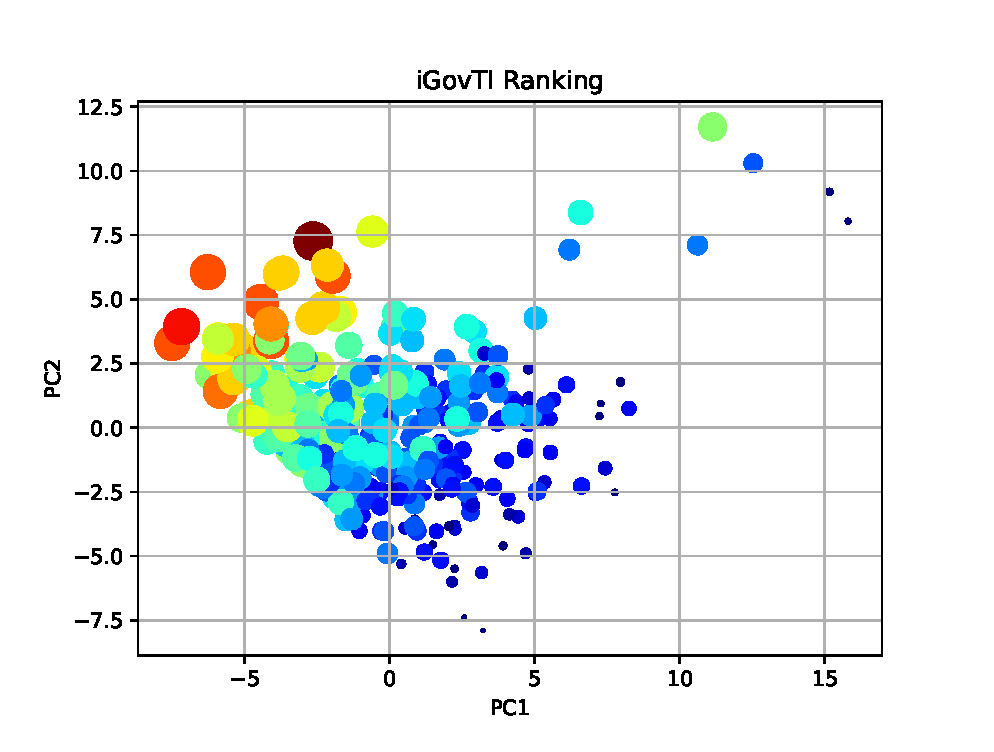
\includegraphics[height=6cm, width=9cm]{figures/pca-svm-rfe_raw_igovti_ranking_pc2.eps}
     \caption{iGovTI ranking from 2 principal components.}
     \label{fig:fig1}
\end{figure}

No Gráfico 2, para analisar apenas a , projetam-se os pontos sobre o eixo da e se tem três grupos (V, II e I). O mesmo processo se aplica a analise da . Assim, observam-se três grupos (V, IV e III). Para cada grupo se seleciona apenas uma variável representativa, o restante é desconsiderado, uma vez que cada grupo significa correlação.
Para o grupo I, tomam-se as variáveis Q16d, Q16e e Q16f que são descorrelacionadas, já no grupo II a questão Q16g é questão selecionada. Ambos os grupos não apresentam FCS. Essas questões denotadas Q16, referem-se a Subdimensão 1.6 (A Alta Administração Utilizou Informações Fornecidas pela Auditoria Interna). Tal subdimensão verifica a participação da auditoria interna das instituições para o preenchimento do questionário. 
% Já no grupo III, que não tem FCS, a variável Q53_Relev é a selecionada; precedidas do grupo IV que também não apresenta FCS. Ressalta-se que ambas as questões apuram a relevância de determinado item. Pela análise ACP, o grupo V mostra as questões que não são representadas pelas  e , é justamente este grupo que contem os FCS.
Depois, buscou-se por meio da análise das ,  e a identificação de FCS (Gráfico 3). O Gráfico 3 mostra a análise dessas componentes principais que revela a existência de três grupos. 

A análise do Gráfico 3 mostra revela a existência de três grupos (VI, VII e VIII). O grupo I contém a variável Q51l que corresponde a FCS e o grupo II também mostra FCS, a variável Q23b.
Na identificação das variáveis significativas das primeiras 20 componentes principais, com os autovalores superiores a 1, as questões que mais contribuem são Q16b (para responder às questões do grupo 2. Estratégias e planos), Q16c (para responder às questões do grupo 3. Informação e conhecimento), Q16d (para responder às questões do grupo 4. Pessoas), Q16e (para responder às questões do grupo 5. Processos) e Q16f (para responder às questões do grupo 6. Resultados da gestão), todas da dimensão “Governança corporativa e de TI, a alta administração utilizou informações fornecidas pela auditoria interna (ou instância equivalente)”. Nota-se que as variáveis Q16, citadas anteriormente, fazem parte do grupo I do Gráfico 2. Ao total foram identificadas 29 variáveis dos 20 primeiras componentes principais (autovalores maiores que 1) das variáveis com significância maior que 0,7. O Quadro 8 mostra quais são essas variáveis significativas. 

No Quadro 8, verificou-se as variáveis que são FCS, de acordo com resultado da pesquisa apresentada na Subseção 4.1. Das 30 questões apenas 5 são FCS, de acordo com classificação obtida por meio de pesquisa qualitativa, quais sejam: Q12c (designou representantes de todas as áreas relevantes para o negócio institucional para compor o Comitê de TI); Q23b (a instituição aprovou e  publicou PDTI interna e externamente); Q51l (gestão de configuração de ativos); Q53e (formalizou a política corporativa de segurança da informação); Q57h (os pagamentos são feitos em função da mensuração objetiva dos resultados entregues e aceitos.
Ainda no Quadro 8, chama-se atenção as ,  e. Nelas constam variáveis com valor positivo ou negativo. Tal fato significa que quanto maior for a resposta de uma questão menor será a da outra. Frisa-se que isto só vale para questões que estejam em uma mesma variável ACP. Caso as questões tenham sinais diferentes (i.e. os elementos dos autovetores), mas em ACP diferentes o sinal positivo e negativo não importa. 
A análise das categorias (Quadro 5) relacionadas às variáveis revela: Q53e referente à Categoria Processos de Gestão de Serviços de TI em Desenho do Serviço que mostrou porcentual igual a 53,85\%; Q57h se liga à Categoria Gestão de Contratos que teve porcentual de 38,46\%; Q23b se vincula à Categoria PDTI que teve 38,46\%. A variável Q51l se relaciona à Categoria Processos de Gestão de Serviços de TI em Transição de Serviços com 19,23\%.
Devido ao baixo percentual de 16,66\% de identificação de FCS do Quadro 8, realizou-se a análise das variáveis que completam as 51 componentes principais, referentes aos 51 autovalores do Quadro 7. Nesta identificação, foram identificadas 33 variáveis, sendo que 8 são FCS, 24,24\% (Quadro 9). Somando os totais obtidos pelo Quadro 8 e pelo se tem, 20,63\% de variáveis que são FCS.

Já o Gráfico 4 mostra a caixa de seleção de variáveis e comandos para ACP em que se utilizam os fatores 1 e 2, eixo x e eixo y respectivamente. O objetivo deste gráfico é fazer os planos principais com a nuvem de pontos dos indivíduos, no caso as 349 instituições.  

O Gráfico 4 representa a relação entre os 2 principais componentes, que representam as questões ou variáveis com maiores autovalores, assim cada ponto representa a relação entre uma instituição e seus 2 principais componentes obtidos por meio de ACP. Cada ponto deste gráfico representa a classificação da instituição em relação a sua classificação no iGovTI de 2012. A partir do resultado apresentado no gráfico 4 é possível identificar um padrão formado pela localização dos componentes principais das organizações com maior índice, onde as organizações com maior iGovTI tiveram valores relativamente semelhantes para seus 2 componentes principais, entretanto ainda não é possível obter uma separação clara entre os resultados. Fazendo-se um corte no eixo das abcissas, a partir do ponto (-8,8, 0), destacam-se 23 instituições à esquerda desse ponto (Quadro 5). 

Dessas instituições, 22, são consideradas pelo TCU como aprimoradas, ou seja, 95,65\%. Apenas a instituição 346 é avaliada como intermediária.
Após a análise ACP, verifica-se que a mesma não é útil para a análise da Hipótese 2. Para responder a essa hipótese, é necessária a execução dos algoritmos de classificação da Subseção 4.4 e da Subseção 4.5.

\subsection{Máquinas de Vetores de Suporte}

Para prever a classificação de uma instituição de acordo com suas respostas para as questões do questionário iGovTI, foram avaliados algoritmos de classificação que pudessem apresentar acurácia para a classificação de organizações de acordo com o iGovTI. Uma vez encontrado um algoritmo capaz desta classificação, é possível utilizar o algoritmo selecionado em conjunto com técnicas de feature selection para identificar as questões mais relevantes para a classificação da instituição de acordo com o iGovTI.
Assim, para a definição do algoritmo de classificação foram realizados testes em 21 algoritmos, a seguir é apresentada uma listagem dos algoritmos avaliados e a taxa de acerto de classificação obtida: 

k-nearest neighbors \cite{fukunaga1975branch}	0.714286
Elastic Net \cite{zou2005regularization}	0.831531
Lasso \cite{tibshirani1996regression}	0.827440
LinearRegression \cite{draper2014applied}	0.360878
LogisticRegression \cite{hosmer2013applied}	0.771429
LDA \cite{martinez2001pca}	0.628571
SVM \cite{hearst1998support}	0.914286
SVM Regression \cite{smola2004tutorial}	0.826885
Linear SVM \cite{fan2008liblinear}	0.714286

O algoritmo que obteve maior sucesso para classificação foi o SVC, que é uma implementação de Máquina de Vetores de Suporte aplicado para a classificação. SVC apresentou uma taxa de acerto de 91,4\%. Para a avaliação dos algoritmos, utilizamos uma metodologia que divide os dados dos questionários pelo iGovTI entre questões que serão utilizadas para aprendizado do algoritmo e questões que serão utilizadas para comparativo de predições. Para treinar o algoritmo utilizou-se 90\% dos dados e os 10\% restantes foram utilizados para avaliar a eficiência de classificação dos algoritmos, comparando a taxa de acerto entre as predições feitas e os valores reais de classificações de organizações pelo iGovTI. 

Uma vez identificado um algoritmo capaz de efetuar a classificação desejada, o próximo passo é identificar as variáveis mais relevantes para esta classificação. Para isso, será utilizado o algoritmo ERV. 

A ERV pode usar vários algoritmos de classificação como critério de seleção das variáveis mais importantes, escolhemos o algoritmo SVC por ele ter apresentado maior acurácia entre os algoritmos de classificação avaliados. Ainda é necessário definir o quantitativo de variáveis mais importantes a serem selecionadas. A partir da pesquisa de identificação por meio de entrevistas na APF, identificou-se 54 variáveis consideradas FCS, este critério foi utilizado para determinar o quantitativo de variáveis mais importantes para a classificação.

Assim, aplicaram-se o algoritmo ERV utilizando o SVC como critério para a seleção das variáveis mais importantes para a classificação, selecionando as 54 variáveis que correspondem aos FCS levantados nas entrevistas com os executivos de TI. Os resultados mostraram que 69,9\% das variáveis foram classificadas da mesma forma que os FCS identificados anteriormente (Quadro 10) por meio de pesquisa qualitativa.

\section{Conclusion}
\label{sec:conclusion}

pca make possible visual discriminative analysis of reduced dataset but it is not easy make correlation betwee extracted features and its original, therefore it is necessary adictional techniques to identify CSF.

SVM have been shown to generalize well even for small sample classification[8]. SVM presents high performance to reproduce the iGovTI classification and can be used for RFE in order to identify CSF

The selected features revealed by RFE are quite similar to the qualitative analysis of Ramos \emph{et al} \cite{ramos2016information}.
\include{chapters/appendix/c_tensor_denoising/c_tensor_denoising}

\bibliographystyle{natbib}
\addcontentsline{toc}{chapter}{Bibliography}
\bibliography{references}

\clearpage
\addappheadtotoc

\end{document}